\documentclass[11pt]{article}

\usepackage[T1]{fontenc}
\usepackage[utf8]{inputenc}
\usepackage[margin=1in]{geometry}
\usepackage{amsmath,amssymb}
\usepackage{graphicx}
\usepackage{booktabs}
\usepackage{longtable}
\usepackage{array}
\usepackage{calc}
\usepackage[hidelinks]{hyperref}

% pandoc list spacing
\providecommand{\tightlist}{%
  \setlength{\itemsep}{0pt}\setlength{\parskip}{0pt}}

\title{Computing the entropy rate of a\\ quantized stationary Gaussian process}
\author{Jeremy Magland\thanks{Center for Computational Mathematics, Flatiron Institute, Simons Foundation, New York, New York 10010}}
\date{}

\begin{document}

\maketitle

\begin{abstract}
We consider a stationary Gaussian process observed after uniform quantization, that is, after rounding each sample to the nearest multiple of a fixed step size. The entropy rate of the resulting integer sequence is the fundamental limit on lossless compression of the quantized signal. This quantity has no closed form, since the probability of a block of quantized values is a high-dimensional Gaussian integral over a box. Furthermore, the classical high-resolution approximation breaks down whenever the spectral density is small or vanishing on part of the spectrum, a situation that arises routinely from ordinary smoothing and filtering operations. In this paper we present two methods for computing the entropy rate. The first is an analytical approximation obtained by combining an exact dithering identity with the Kolmogorov--Szegő formula. In this approximation the quantization noise power acts as a floor on the spectral density, so that the rate remains finite in situations where the classical formula fails. The second method is a Monte Carlo estimate of the exact rate. The process is represented as a finite moving average of independent Gaussian innovations using its minimum-phase spectral factor. The quantized sequence is then a hidden Markov process, for which the optimal (fully adapted) particle filter may be written in closed form. By the Shannon--McMillan--Breiman theorem, the entropy rate may be estimated by evaluating the filter's log-likelihood on a single long sequence drawn from the process. The Monte Carlo method may be used directly, or as a means of assessing the accuracy of the analytical approximation. In numerical experiments across a range of process families, the approximation agrees with the Monte Carlo estimate to within a few millibits per sample for quantization steps up to the standard deviation of the signal, including strongly filtered processes for which the classical formula fails outright. We also compare selected lossless coders against the computed limit. In target scenarios of interest, linear predictive coding followed by an entropy coder comes within a few percent of the entropy rate, whereas a general-purpose byte-oriented compressor applied to the raw samples remains far from the limit. A reference implementation in Python is available.
\end{abstract}

\section{Introduction}\label{introduction}

The entropy rate of a quantized stationary Gaussian process arises in the study of the compressibility of noisy signals. When a continuous-valued signal is digitized using uniform quantization, the resulting integer sequence is what is actually stored, and its entropy rate is the fundamental limit on lossless compression, that is, the number of bits per sample that the signal actually carries.

Let \(\{X_t\}_{t\in\mathbb Z}\) be a zero-mean stationary Gaussian process with autocovariance \(\gamma_k = \mathbb E[X_t X_{t+k}]\), spectral density \(S(\omega) = \sum_k \gamma_k e^{-ik\omega} \ge 0\) on \([-\pi,\pi]\), and variance \(\sigma^2 = \gamma_0\). The process is quantized with step \(\Delta > 0\):
\[Y_t = \operatorname{round}(X_t/\Delta) \in \mathbb Z,\]
so that \(Y_t = y\) if and only if \(X_t\) lies in the cell \(\mathcal C_y = [(y-\tfrac12)\Delta,\,(y+\tfrac12)\Delta)\). The quantity of interest is the entropy rate, in bits per sample,
\[\bar H = \lim_{n\to\infty}\frac1n H(Y_1,\dots,Y_n), \qquad H(Y_1^n) = -\sum_{y\in\mathbb Z^n} P(Y_1^n = y)\,\log_2 P(Y_1^n = y).\]
Although the alphabet is countably infinite, \(\bar H\) is finite because \(X_t\) has finite variance.

Computing \(\bar H\) accurately is difficult. The definition requires the log-probabilities of individual quantization cells, and each such probability is a high-dimensional Gaussian integral over a box. When the spectral density takes values close to zero at some frequencies, the underlying covariance matrix is nearly singular and these integrals become very challenging to compute accurately. The ill-conditioned situation is common in practice as it arises from Gaussian smoothing, from lowpass, highpass, and bandpass filtering, and even from a simple moving average.

This paper makes two contributions. The first is an analytical approximation. An exact dithering identity converts the discrete entropy into a Riemann sum for the differential entropy of the dithered process \(X + U\), whose spectral density is exactly \(S(\omega) + \Delta^2/12\); applying the Kolmogorov--Szegő formula then yields
\[\bar H \;\approx\; \frac{1}{4\pi}\int_{-\pi}^{\pi}\log_2\frac{2\pi e\,\big(S(\omega)+\Delta^2/12\big)}{\Delta^2}\,d\omega.\]
This is the classical high-resolution formula, except with an added term representing the noise power of the quantizer. The modified formula is finite for any spectral density, since its integrand is bounded below. Whether it is also accurate is not settled by the derivation, and we address the question empirically in Section 5, using the Monte Carlo estimator described below as ground truth. Across the process families studied there, including strongly filtered processes for which the classical formula fails, the approximation agrees with the exact rate to within a few millibits per sample for quantization steps up to about the standard deviation of the signal; for substantially coarser steps the approximation breaks down and the estimator should be used instead.

The second contribution is a Monte Carlo estimator of the exact rate. By writing \(X_t\) as a finite moving average of i.i.d. Gaussian innovations using its minimum-phase spectral factor, the process \(\{Y_t\}\) becomes a hidden Markov process for which the optimal (fully adapted) particle filter is available in closed form. Running the filter on a single long typical sequence and invoking the Shannon--McMillan--Breiman theorem gives an estimate of \(\bar H\) that converges as the particle count and the sequence length grow together, approaching the true rate from above. The estimator may be used directly, or as a means of evaluating the accuracy of the analytical approximation across a range of settings.

The individual ingredients (high-resolution quantization theory \cite{GrayNeuhoff1998}, dithered quantization \cite{GrayStockham1993,ZamirFeder1996}, the Kolmogorov--Szegő formula \cite{GrenanderSzego1958}, and particle filtering \cite{PittShephard1999}) are all well established. The closest prior work on the approximation is that of Zamir and Feder \cite{ZamirFeder1996}, who analyzed the information rates of dithered uniform quantizers applied to filtered Gaussian sources; the noise power \(\Delta^2/12\) enters their analysis in essentially the role it plays in the formula above. Their subject, however, is a genuinely dithered system, characterized in rate--distortion terms, whereas here the dither is purely an analytical device, introduced through the exact identity of Section 3.1, and the quantity approximated is the entropy rate of the undithered quantizer output at finite \(\Delta\). Geiger and Koch \cite{GeigerKoch2019} studied the entropy rate of the same undithered process in the fine-quantization limit: normalizing by \(\log(1/\Delta)\) and letting \(\Delta \to 0\), they showed that the limit, which they call the information dimension rate, equals the fraction of the band on which the spectral density is positive. Their proof likewise employs a dithering identity and the noise floor \(\Delta^2/12\), but the normalization retains only the leading term. To our knowledge the approximation formula above, as a finite-\(\Delta\) description of the undithered quantizer, has not previously appeared. On the computational side, the reduction of an information rate to the log-likelihood of a filter evaluated on a single long typical sequence is well established for channels with memory: Arnold et al.\ \cite{ArnoldEtAl2006} developed the approach for finite-state channels using the exact forward recursion, and Dauwels and Loeliger \cite{DauwelsLoeliger2008} extended it to continuous-state models by particle methods. The contribution of Section 4 is the application of this construction to the uniformly quantized stationary Gaussian process, for which the minimum-phase moving-average representation makes the optimal (fully adapted) particle filter available in closed form.

The paper is organized as follows. Section 2 reviews the classical high-resolution formula and describes the situations in which it fails. Section 3 derives the analytical approximation. Section 4 presents the particle-filter estimator together with its diagnostics. Section 5 reports numerical experiments, Section 6 describes the accompanying implementations, and Section 7 concludes with a discussion of limitations and future work.

\section{The classical high-resolution formula and its failure}\label{the-classical-high-resolution-formula-and-its-failure}

For small \(\Delta\), the classical approach assumes that the density \(f\) of \(X_1^n\) is approximately constant over each quantization cell \cite{GrayNeuhoff1998}, so that
\[P(Y_1^n = y) = \int_{\prod_t \mathcal C_{y_t}} f(x)\,dx \;\approx\; \Delta^n f(\Delta y).\]
Substituting into the entropy sum and recognizing a Riemann sum with spacing \(\Delta\) \cite[Ch.~8]{CoverThomas2006},
\[H(Y_1,\dots,Y_n) \;\approx\; -\sum_{y\in\mathbb Z^n}\Delta^n f(\Delta y)\,\log_2 f(\Delta y) - n\log_2\Delta \;\approx\; h(X_1^n) - n\log_2\Delta,\]
where \(h\) denotes differential entropy in bits. Since \(X\) is exactly Gaussian, the Kolmogorov--Szegő formula gives its differential entropy rate directly, and dividing by \(n\) and letting \(n\to\infty\) we obtain

\[\bar H_{\mathrm{classical}} \;=\; \tfrac12\log_2(2\pi e) + \frac{1}{4\pi}\int_{-\pi}^{\pi}\log_2 S(\omega)\,d\omega - \log_2\Delta \;=\; \frac{1}{4\pi}\int_{-\pi}^{\pi}\log_2\frac{2\pi e\,S(\omega)}{\Delta^2}\,d\omega.\]

The problem with this formula is apparent: the integrand contains \(\log_2 S(\omega)\), which diverges to \(-\infty\) wherever \(S(\omega)\to 0\). If the spectral density vanishes, or is merely very small, on a portion of the frequency axis, the classical formula predicts an arbitrarily negative entropy rate, which is impossible since \(H(Y_1^n) \ge 0\). The failure can be traced to the constant-density approximation: when the spectral power is small, certain linear combinations of the samples have standard deviations far below \(\Delta\), and \(f\) is therefore far from constant across a single cell in those directions.

As noted in the introduction, spectra of this kind arise readily in practice. Any linear operation that strongly attenuates part of the spectrum, including Gaussian smoothing, lowpass, highpass, and bandpass filtering, and even a simple moving average, drives \(S\) toward zero on a set of frequencies and puts the classical formula out of reach.

The fine-quantization behavior in this regime is known. Geiger and Koch \cite{GeigerKoch2019} showed that \(\bar H/\log_2(1/\Delta)\) converges, as \(\Delta \to 0\), to the fraction of the band on which \(S\) is positive, a quantity they call the information dimension rate of the process. What is missing is a description at finite \(\Delta\), as happens in the case of a real measured signal, and this is the subject of the next section.

\section{The analytical approximation}\label{the-analytical-approximation}

The derivation follows the same outline as in Section 2, except that the cell probabilities are expressed exactly rather than approximately, by way of an identity relating them to the density of a dithered version of the process.

\subsection{The dither identity}\label{the-dither-identity}

Let \(U_t \sim \mathrm{Unif}(-\Delta/2,\Delta/2)\), i.i.d. and independent of \(X\). With \(f\) the density of \(X_1^n\), the density \(g\) of \(X_1^n + U_1^n\) is
\[g(u) = \Delta^{-n}\int_{\prod_t [u_t - \Delta/2,\; u_t + \Delta/2]} f(x)\,dx.\]
Substituting \(u = \Delta y\) for \(y\in\mathbb Z^n\) gives
\[P(Y_1^n = y) = \Delta^n\,g(\Delta y).\]
In other words, the probability of observing the quantized output \(y\) is exactly equal to the density of the dithered process \(X + U\) evaluated at the lattice point \(\Delta y\), multiplied by the cell volume \(\Delta^n\); identities of this kind are standard in the analysis of dithered quantization \cite{GrayStockham1993}.

\subsection{The Riemann-sum step and its lattice error}\label{the-riemann-sum-step-and-its-lattice-error}

The differential entropy of \(g\) is
\[h(X_1^n + U_1^n) = -\int_{\mathbb R^n} g(u)\,\log_2 g(u)\,du,\]
which is approximately equal to its Riemann sum with spacing \(\Delta\):
\[h(X_1^n + U_1^n) \approx -\sum_{y\in\mathbb Z^n}\Delta^n\,g(\Delta y)\,\log_2 g(\Delta y).\]
Substituting \(\Delta^n g(\Delta y) = P(Y_1^n = y)\), the right-hand side equals \(H(Y_1^n) + n\log_2\Delta\), so that
\[H(Y_1,\dots,Y_n) \;\approx\; h(X_1^n + U_1^n) - n\log_2\Delta.\]
Writing \(F(u) = -g(u)\log_2 g(u)\), the Poisson summation formula gives
\[\varepsilon_{\mathrm{lat}}^{(n)} \;:=\; h(X_1^n + U_1^n) - n\log_2\Delta - H(Y_1,\dots,Y_n) \;=\; -\sum_{k\in\mathbb Z^n\setminus\{0\}}\hat F(2\pi k/\Delta), \qquad \hat F(\xi) = \int_{\mathbb R^n} F(u)\,e^{-i\xi\cdot u}\,du.\]
The error is thus a sum of Fourier coefficients of \(F\) evaluated at the nonzero reciprocal lattice points \(2\pi k/\Delta\), which recede to infinity as \(\Delta\to 0\). Its magnitude depends on the rate of decay of \(\hat F\), that is, on the smoothness of \(g\log_2 g\). If \(F\) has \(p\) integrable derivatives then the error is \(O(\Delta^p)\), and for smooth \(F\) it decays faster than any power of \(\Delta\). We do not pursue this analysis here.

\subsection{The spectrum of the dithered process and the Kolmogorov--Szegő step}\label{the-spectrum-of-the-dithered-process-and-the-kolmogorovszegux151-step}

\(U_t\) is i.i.d. with mean zero and variance \(\frac1\Delta\int_{-\Delta/2}^{\Delta/2}u^2\,du = \Delta^2/12 =: v\), so its spectral density is the constant \(v\). Since \(U\) is independent of \(X\), the spectral densities add, and \(X + U\) has spectral density exactly \(S(\omega) + v\).

We approximate \(X + U\) by the Gaussian process with the same spectral density. By the Kolmogorov--Szegő formula \cite{GrenanderSzego1958}, a stationary Gaussian process with spectral density \(S_d\) has differential entropy rate

\[\tfrac12\log_2(2\pi e) + \frac{1}{4\pi}\int_{-\pi}^{\pi}\log_2 S_d(\omega)\,d\omega.\]

Since the Gaussian maximizes entropy for a given covariance \cite{CoverThomas2006}, this is an upper bound on the differential entropy rate of \(X + U\).

Combining these steps, we divide \(H(Y_1^n) \approx h(X_1^n + U_1^n) - n\log_2\Delta\) by \(n\), let \(n\to\infty\), and substitute \(S_d = S + v\):
\[\boxed{\;\bar H \;\approx\; \frac{1}{4\pi}\int_{-\pi}^{\pi}\log_2\frac{2\pi e\,\big(S(\omega)+\Delta^2/12\big)}{\Delta^2}\,d\omega.\;}\]
This is the classical formula of Section 2 with \(S\) replaced by \(S + v\), and the replacement repairs the failure identified there. Since the spectrum is bounded below by \(v = \Delta^2/12\), the integrand saturates at \(\log_2(2\pi e\,v/\Delta^2) = \log_2(2\pi e/12)\) at frequencies where \(S \ll v\), rather than diverging.

Note that the formula also recovers the fine-quantization limit of Geiger and Koch \cite{GeigerKoch2019} described in Section 2: as \(\Delta \to 0\) the integrand grows like \(2\log_2(1/\Delta)\) at frequencies where \(S > 0\) and tends to the constant \(\log_2(2\pi e/12)\) where \(S = 0\), so that the right-hand side divided by \(\log_2(1/\Delta)\) converges to the information dimension rate. In other words, the approximation is not merely finite in the situations where the classical formula fails; its leading behavior there is correct.

\subsection{Sources of error}\label{sources-of-error}

Only two approximations were made in the derivation; the remaining steps are exact.

The first is the lattice error \(\varepsilon_{\mathrm{lat}}^{(n)}\) from the Riemann-sum step, given exactly by the Poisson sum above. It is small to the extent that the Fourier coefficients of \(g\log_2 g\) decay rapidly at the reciprocal lattice points; we have not attempted to quantify it here.

The second is the error of the Gaussian approximation: \(X + U\) is not Gaussian (\(U\) is uniform), and the Kolmogorov--Szegő rate for the spectral density \(S + v\) is an upper bound on the true differential entropy rate. The slack in this bound is the per-sample non-Gaussianity of \(X + U\), which is small since the uniform component is a small perturbation of the Gaussian. Note that this error always acts in the same direction: the formula overestimates \(\bar H\).

\subsection{Domain of validity}\label{domain-of-validity}

The approximation remains accurate well into the coarse-quantization regime. It fails only when \(\Delta\) is much larger than the scale of the signal itself. In that extreme regime the formula tends to the constant floor \(\tfrac12\log_2(2\pi e/12)\) while the true rate tends to zero; this is an artifact of modeling rounding as additive noise. The value of the floor, approximately \(0.25\) bits, is a familiar constant of high-resolution quantization theory, being the asymptotic excess of entropy-coded uniform quantization over the rate--distortion function \cite{GrayNeuhoff1998,GishPierce1968}. Such extreme quantization is not typical of applications, however. In practice the standard deviation of the signal is at least about twice the quantization step, which is comfortably within the range of validity. Section 5 maps the accuracy of the approximation empirically, using the estimator of Section 4 as ground truth.

\section{The particle-filter estimator}\label{the-particle-filter-estimator}

The approximation of Section 3 involves two error terms that have not been quantified, and an independent method for computing the exact rate is therefore needed, both for direct use and for assessing the accuracy of the approximation.

\subsection{Reduction to one typical sequence}\label{reduction-to-one-typical-sequence}

Since \(\{Y_t\}\) is stationary and ergodic (it is a pointwise function of an ergodic Gaussian process, and ergodicity holds provided \(S\) has no atoms), the Shannon--McMillan--Breiman theorem \cite{CoverThomas2006,Chung1961} gives
\[\bar H = \lim_{n\to\infty} -\tfrac1n \log_2 P(Y_1^n) \quad \text{a.s.}\]
Note that the alphabet here is countably infinite, so the usual finite-alphabet statement of the theorem does not literally apply; the extension to countable alphabets is due to Chung \cite{Chung1961}, and its hypothesis \(H(Y_1) < \infty\) is satisfied because \(X_t\) has finite variance, as noted in Section 1. Thus the problem reduces to computing the log-likelihood of a single long typical sequence \(y_1^n\) drawn from the process itself.

\subsection{Moving-average model and hidden Markov structure}\label{moving-average-model-and-hidden-markov-structure}

We represent \(X_t\) as a finite moving average of i.i.d. standard Gaussian innovations:
\[X_t = \sum_{j=0}^{L-1} h_j\,W_{t-j}, \qquad W_t \overset{\text{iid}}{\sim}\mathcal N(0,1),\]
with taps \(h\) chosen so that the model autocovariance \(\gamma^h_k = \sum_j h_j h_{j+k}\) matches the target \(\gamma_k\) (equivalently \(|\hat h(\omega)|^2 = S(\omega)\)), taking \(L\) several times the correlation length. Among the possible spectral square roots we choose the minimum-phase factor, which is computed using the standard cepstral construction \cite[Ch.~13]{OppenheimSchafer2010} (see the implementation of Section 6). This choice is important for the filtering application since it maximizes the leading tap, giving
\[h_0^2 = \exp\!\Big(\tfrac{1}{2\pi}\int_{-\pi}^{\pi}\ln S(\omega)\,d\omega\Big),\]
the one-step prediction error variance (Szegő). We assume throughout that \(\int_{-\pi}^{\pi}\ln S(\omega)\,d\omega > -\infty\), so that \(h_0 > 0\); a process whose spectral density vanishes on a set of positive measure is perfectly predictable from its past and admits no such representation. Since \(h_0\) is the conditional standard deviation of \(X_t\) given the past innovations, a symmetric (zero-phase) square root, for which the leading tap is very small, would render the filter degenerate.

Because \(X_t\) depends only on \((W_{t-L+1},\dots,W_t)\), the process \(\{Y_t\}\) is a hidden Markov process with continuous state \(u_t = (W_{t-L+2},\dots,W_t)\in\mathbb R^{L-1}\). The likelihood factors as \(\log_2 P(y_1^n) = \sum_t \log_2 P(y_t\mid y_1^{t-1})\), and each predictive probability is estimated using a particle filter.

\subsection{The fully adapted filter}\label{the-fully-adapted-filter}

The structure of the model admits the optimal (fully adapted) particle filter \cite{PittShephard1999} in closed form. Given the past innovations \(u\), we have \(X_t = h_0 W_t + \mu\) with \(\mu = \sum_{j=1}^{L-1} h_j u_{t-j}\) and \(W_t \sim \mathcal N(0,1)\) independent of the past. Writing \(\Phi\) for the standard normal CDF and expressing the observed cell in standardized units,
\[l = \frac{(y_t-\tfrac12)\Delta - \mu}{h_0}, \qquad r = \frac{(y_t+\tfrac12)\Delta - \mu}{h_0}, \qquad r - l = \frac{\Delta}{h_0},\]
we see that the observation probability is a Gaussian cell probability, \(P(Y_t = y_t \mid u) = \Phi(r) - \Phi(l)\), and that conditional on \(\{Y_t = y_t\}\) and \(u\), the new innovation \(W_t\) is \(\mathcal N(0,1)\) truncated to \([l, r)\).

Note that the dimensionless ratio \(\Delta/h_0\), the quantization step divided by the one-step prediction error, is the key parameter: \(\Delta/h_0 \gg 1\) corresponds to coarse quantization and \(\Delta/h_0 \ll 1\) to fine quantization.

Each of \(N\) particles stores the last \(L-1\) innovations. Resampling is performed at every step, which keeps the weights uniform, so the predictive estimate is a plain average.

\begin{quote}
\textbf{Algorithm.}

\textbf{Inputs:} taps \(h_0 > 0, h_1, \dots, h_{L-1}\); step \(\Delta\); sequence \(y_1^n \in \mathbb Z^n\); particle count \(N\).

Initialize \(u^{(i)}_{2-L},\dots,u^{(i)}_0 \overset{\text{iid}}{\sim} \mathcal N(0,1)\) for each \(i\) (this is the exact prior, so no burn-in is needed). Set \(\ell \leftarrow 0\) (accumulated in nats).

For \(t = 1,\dots,n\):

\begin{enumerate}
\def\labelenumi{\arabic{enumi}.}
\tightlist
\item
  \textbf{Weights:} for each \(i\): \(\mu^{(i)} = \sum_{j=1}^{L-1} h_j u^{(i)}_{t-j}\); \(\;l^{(i)} = \big((y_t-\tfrac12)\Delta - \mu^{(i)}\big)/h_0\), \(\;r^{(i)} = l^{(i)} + \Delta/h_0\); \(\;\alpha^{(i)} = \Phi(r^{(i)}) - \Phi(l^{(i)})\).
\item
  \textbf{Likelihood increment:} \(\ell \leftarrow \ell + \ln\big(\tfrac1N\sum_i \alpha^{(i)}\big)\).
\item
  \textbf{Resample:} draw ancestor indices by systematic resampling with probabilities \(\propto \alpha^{(i)}\); set each particle's innovation buffer to its ancestor's.
\item
  \textbf{Propagate:} for each \(i\), draw \(u^{(i)}_t \sim \mathcal N(0,1)\) truncated to \([l^{(a_i)}, r^{(a_i)})\).
\end{enumerate}

\textbf{Output:} \(\hat{\bar H} = -\ell/(n\ln 2)\) bits per sample.
\end{quote}

Step 4 samples exactly from \(p(w_t \mid y_t, u)\) and step 3 resamples using the exact predictive weights, so this is the fully adapted auxiliary particle filter for this model, and \(\prod_t \frac1N\sum_i \alpha^{(i)}\) is an unbiased estimator of \(P(y_1^n)\) \cite[Prop.~7.4.1]{DelMoral2004}. The computational cost is \(O(nNL)\) time and \(O(NL)\) memory. Numerically stable evaluation of the cell probabilities and of the truncated-normal draws requires some care in log space; the details are given in Appendix A and in the accompanying code.

\subsection{Bias, convergence, and reporting}\label{bias-convergence-and-reporting}

The estimator overestimates \(\bar H\) in expectation for two reasons. First, by Jensen's inequality, \(\mathbb E\log\hat P(y_1^n) \le \log P(y_1^n)\), since the particle likelihood is unbiased on the natural scale but not on the log scale; the resulting bias is of order \(O(1/N)\) per sample; Section 5.1 observes this rate for processes of moderate difficulty (for the hardest processes the decay is slower at practical particle counts). Second, the finite-\(n\) block entropy \(\tfrac1n H(Y_1^n)\) is non-increasing in \(n\) and converges to \(\bar H\) \cite{CoverThomas2006}. Both effects vanish in the appropriate limit, so that \(\hat{\bar H}\) approaches \(\bar H\) from above and the practical convergence check is to increase \(N\) and \(n\) until the estimate stops decreasing. Results are reported as the mean \(\pm\) standard error over independent replicates, each with a freshly generated sequence and filter, and Section 5 includes a convergence study with respect to both \(N\) and \(n\).

For strongly smoothing processes the particle cloud can lose track of the state entirely, in which case the resulting estimate is not merely noisy but invalid, and the effective sample size does not detect the failure. The failure mode, together with a diagnostic based on the per-step likelihood increment that does detect it, is described in Appendix B.

\section{Numerical experiments}\label{numerical-experiments}

This section reports numerical experiments over a range of process families (white noise, the first difference, moving averages, AR(1), Gaussian smoothing, and lowpass filtering) and quantization steps. Section 5.1 studies the convergence of the particle-filter estimator in its two parameters and establishes how they should be chosen. Section 5.2 then compares the analytical approximation of Section 3 against the resulting estimates across the process families, and, within the validated range, surveys the dependence of the entropy rate on the process and quantization parameters. Finally, Section 5.3 compares practical lossless coders against the estimated rate.

\subsection{Convergence of the particle filter}\label{convergence-of-the-particle-filter}

The estimator of Section 4 has two convergence parameters, the particle count \(N\) and the sequence length \(n\), and the experiments in this subsection establish how they should be chosen. Seven processes spanning the range of difficulty the filter encounters are used, all quantized at \(\Delta = 0.25\sigma\): moving averages of widths 8, 16, 32, and 64, Gaussian smoothing kernels of widths \(\tau = 1\) and \(\tau = 1.25\), and the first difference. Two strongly smoothing processes, for which the filtering problem is hardest, are used to study the collapse diagnostic: a 33-tap windowed-sinc lowpass filter (cutoff 6 kHz at a sampling rate of 30 kHz) at \(\Delta = 0.25\sigma\), and a Gaussian kernel of width \(\tau = 1.5\) at \(\Delta = 0.5\sigma\). All runs used the WebGPU engine described in Section 6, and scripts reproducing every figure and table are included in the repository.

Figure 1 shows the paired excess of the estimate at particle count \(N\) over the estimate at \(N = 128000\) on the same observed sequences. The pairing cancels the sequence-to-sequence variation and isolates the filter bias. The excess is positive throughout and decreases with \(N\) in every process, as expected from the Jensen bias discussed in Section 4.4, and for the processes of moderate difficulty the decay is consistent with the expected \(O(1/N)\) rate over more than two decades.

\begin{figure}[t]
\centering
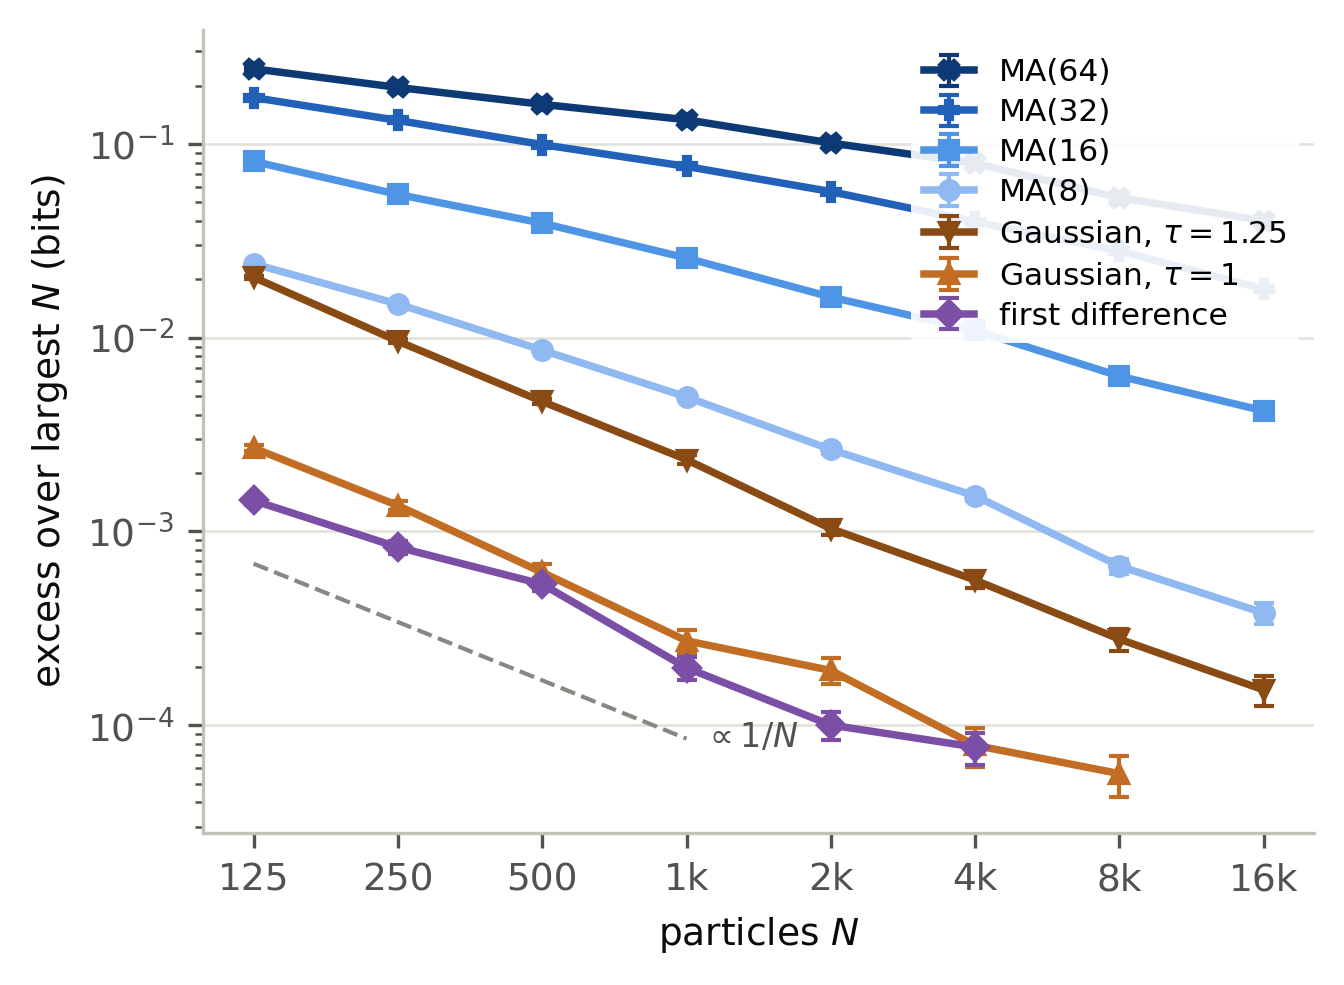
\includegraphics[width=0.7\linewidth]{../experiments/figures/fig_convergence_particles.png}
\caption{Convergence in the particle count $N$: the paired excess of the estimate at $N$ over the estimate at $N = 128000$ on the same observed sequences, at $n = 20000$ with 32 replicates and $\Delta = 0.25\sigma$. Each curve is drawn up to the last $N$ at which the excess is resolved (mean above two standard errors). The dashed guide is proportional to $1/N$; note that the moving-average curves are visibly shallower. Since the reference carries a residual bias of its own, the rightmost points understate the true bias by about 12 percent.}
\label{fig:1}
\end{figure}

The size of the bias at a given \(N\) spans more than two orders of magnitude across the processes, and the variation is evidently not governed by the dimension of the state; the AR(1) process with \(\rho = 0.9\), whose filter carries a 63-dimensional state, is already converged at \(N = 125\) and does not appear in the figure. It is instead related to the structure of the spectrum: the moving averages, whose spectra vanish at the \(w - 1\) nulls of the boxcar response, are the most biased at every width, and for the wider ones the decay is visibly slower than \(1/N\). The \(O(1/N)\) asymptotics presumably still hold, but the particle count at which they set in recedes as the process hardens; the same slow convergence is encountered in Section 5.2. In practice the convergence check of Section 4.4 is inexpensive, and for processes of moderate difficulty a few thousand particles suffice.

Figure 2 shows the corresponding sweep over the sequence length at fixed \(N\). The replicate standard deviation shrinks in proportion to \(1/\sqrt{n}\) for every process across the 64-fold range of lengths, while the means are constant to within their error bars; the finite-\(n\) transient of Section 4.4, which is \(O(L/n)\) of the total, is resolvable only for the widest kernel at the shortest lengths. In other words, the role of \(n\) is to increase precision, while the bias is controlled by \(N\) alone. Since the variance of the reported mean scales as the reciprocal of the total sample count \(rn\), a fixed budget may be divided between longer sequences and more replicates as convenience dictates, provided \(n\) is much longer than the correlation length. The experiments of Section 5.2 exploit this freedom: since every step is an opportunity to lose lock, their hardest points are run as many short replicates rather than a few long ones.

\begin{figure}[t]
\centering
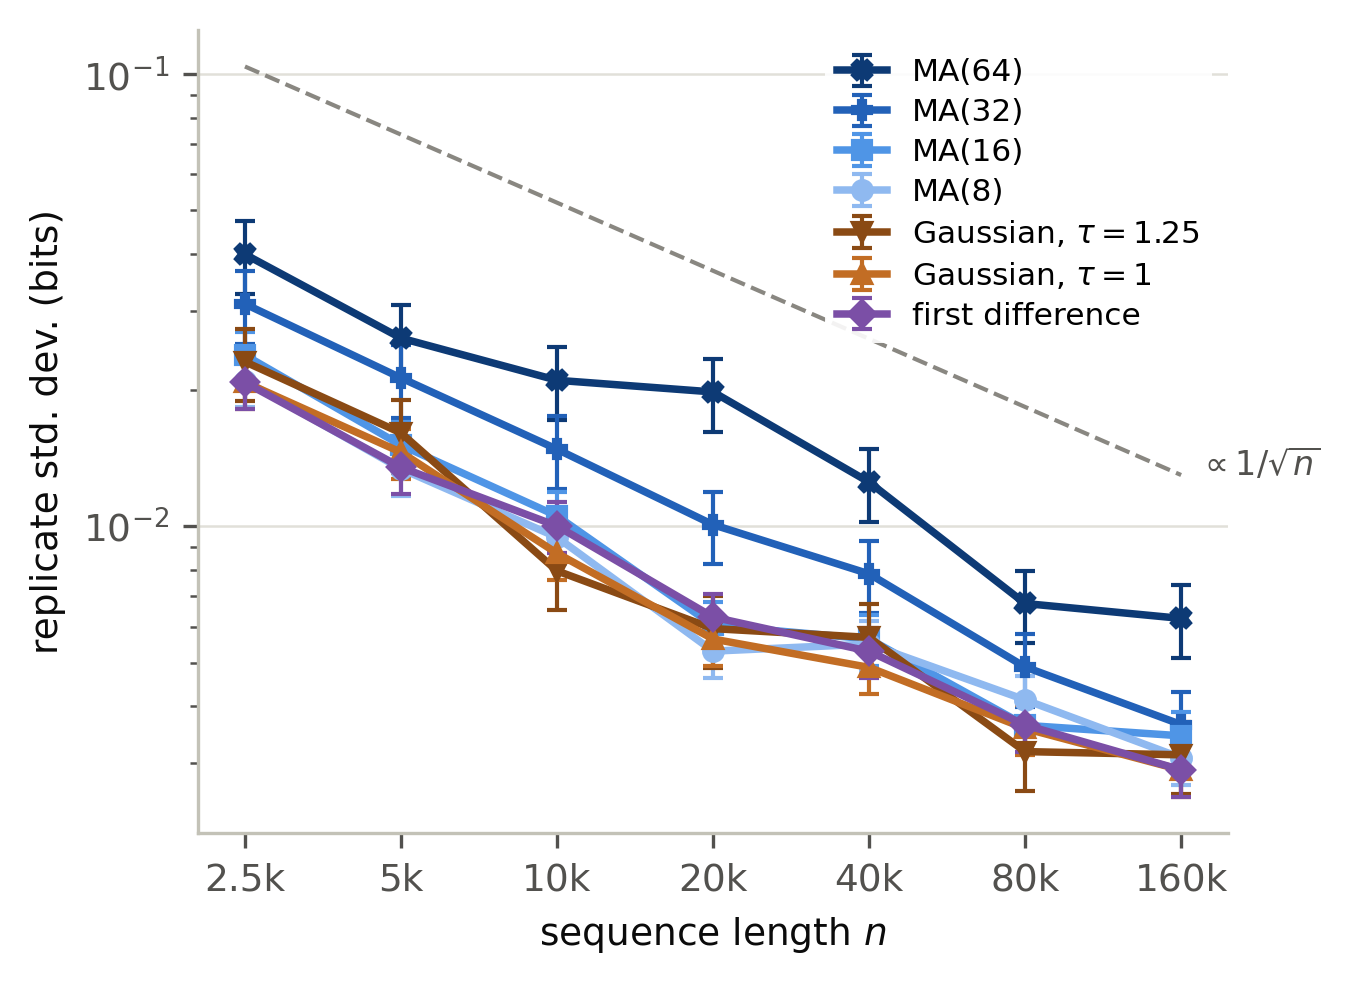
\includegraphics[width=0.7\linewidth]{../experiments/figures/fig_convergence_length.png}
\caption{Convergence in the sequence length $n$: the standard deviation across replicates at fixed particle count ($N = 4000$; $16000$ for the moving averages of widths 32 and 64), with $\Delta = 0.25\sigma$. Error bars are the standard error of the standard deviation (32 replicates; 16 for the two widest moving averages). The dashed guide is proportional to $1/\sqrt{n}$.}
\label{fig:2}
\end{figure}

For the two strongly smoothing processes the picture changes qualitatively. Figure 3 shows, as a function of the particle count, the fraction of steps flagged by the lost-lock diagnostic of Appendix B together with the mean effective sample size, and Table 1 reports the corresponding estimates. At small \(N\) every replicate loses the state, and the resulting values are not merely inaccurate but invalid, exceeding the memoryless upper bound \(H(Y_1)\) by many orders of magnitude. The transition to reliable operation is fairly sharp for the Gaussian kernel, all replicates keeping lock from \(N = 3000\) onward, whereas the lowpass process, whose state has dimension 32, requires \(N = 100000\). Note that each step is an opportunity to lose the state, so the particle count required grows with the sequence length.

\begin{figure}[t]
\centering
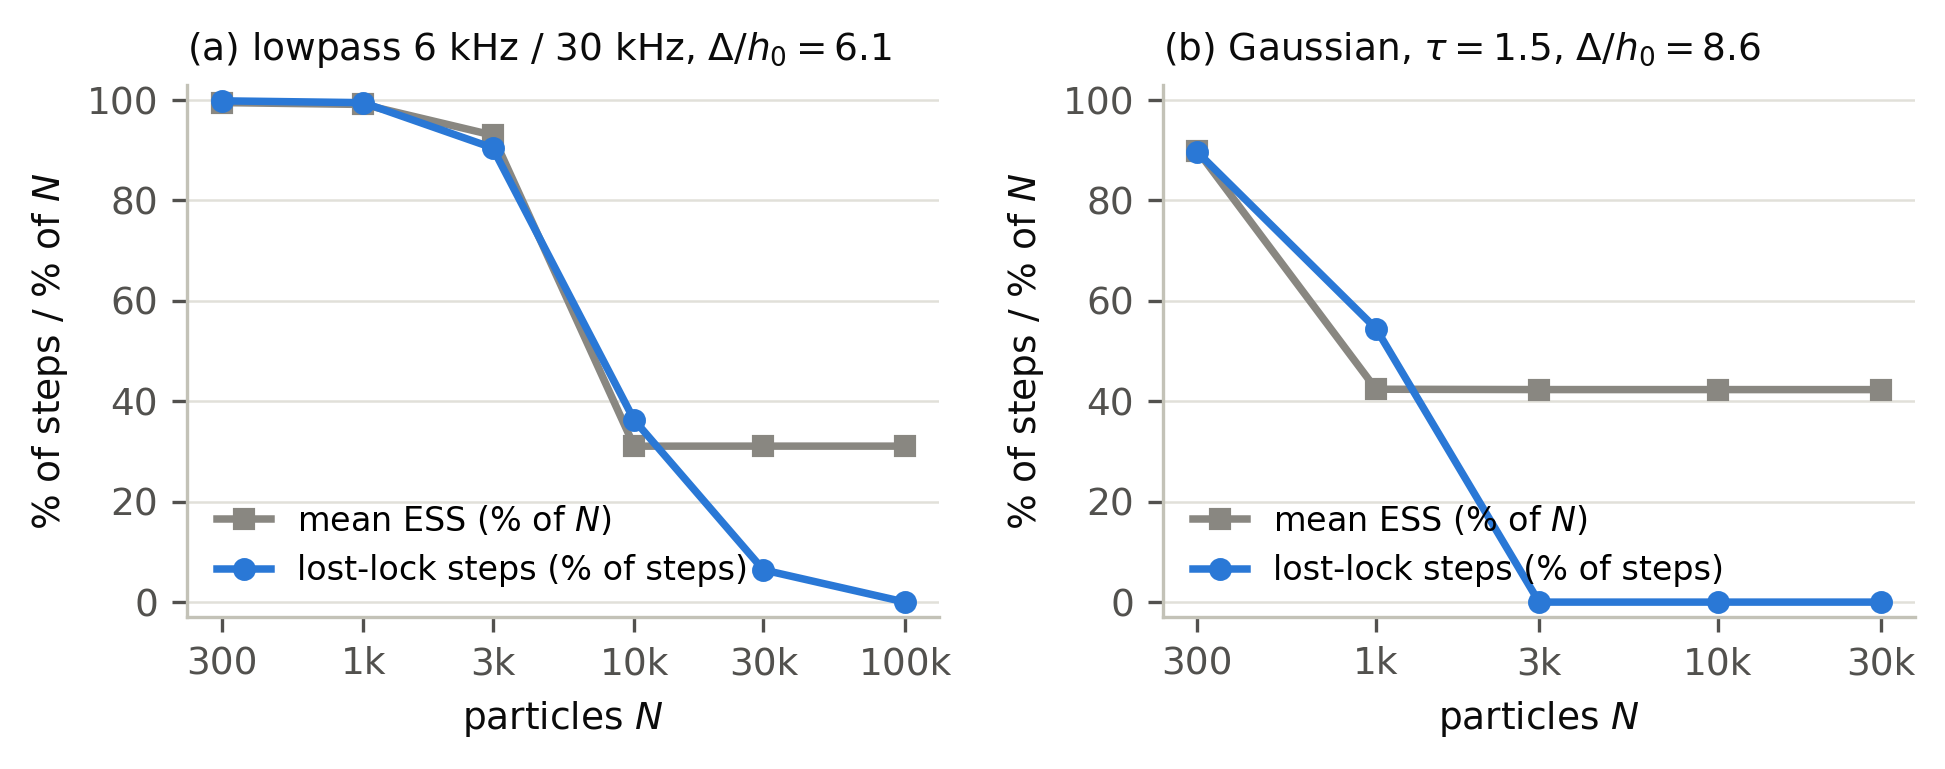
\includegraphics[width=\linewidth]{../experiments/figures/fig_convergence_collapse.png}
\caption{Behavior of the collapse diagnostic in the fine-quantization regime, for (a) the lowpass process at $\Delta = 0.25\sigma$ and (b) the Gaussian kernel with $\tau = 1.5$ at $\Delta = 0.5\sigma$, at $n = 30000$ with eight replicates. Shown are the fraction of steps flagged as lost-lock by the diagnostic of Appendix B and the mean effective sample size as a fraction of $N$. Note that the ESS is highest in the collapsed regime.}
\label{fig:3}
\end{figure}

The effective sample size does not detect these failures; it is in fact higher in the collapsed regime than in the healthy one, since once every particle is comparably far from the true state the weights are nearly uniform and the resampling statistics appear ideal. The per-step log-likelihood diagnostic, by contrast, flags the collapsed steps directly, and the affected replicates are discarded rather than averaged in.

\textbf{Table 1.} The collapse study. A run is \emph{collapsed} when every replicate lost the state, and \emph{provisional} when some but not all did, since the surviving replicates were produced by the same particle count that failed elsewhere. Lost-lock steps and mean ESS are averaged over all replicates, including discarded ones.

\textbf{lowpass 6 kHz / 30 kHz} (\(\Delta = 0.25\sigma\), \(\Delta/h_0 = 6.1\), \(L = 33\), \(n = 30000\)):

\begin{longtable}[]{@{}
  >{\raggedleft\arraybackslash}p{(\linewidth - 8\tabcolsep) * \real{0.2000}}
  >{\raggedleft\arraybackslash}p{(\linewidth - 8\tabcolsep) * \real{0.2000}}
  >{\raggedleft\arraybackslash}p{(\linewidth - 8\tabcolsep) * \real{0.2000}}
  >{\raggedleft\arraybackslash}p{(\linewidth - 8\tabcolsep) * \real{0.2000}}
  >{\raggedleft\arraybackslash}p{(\linewidth - 8\tabcolsep) * \real{0.2000}}@{}}
\toprule\noalign{}
\begin{minipage}[b]{\linewidth}\raggedleft
\(N\)
\end{minipage} & \begin{minipage}[b]{\linewidth}\raggedleft
estimate (bits/sample)
\end{minipage} & \begin{minipage}[b]{\linewidth}\raggedleft
discarded replicates
\end{minipage} & \begin{minipage}[b]{\linewidth}\raggedleft
lost-lock steps
\end{minipage} & \begin{minipage}[b]{\linewidth}\raggedleft
mean ESS
\end{minipage} \\
\midrule\noalign{}
\endhead
\bottomrule\noalign{}
\endlastfoot
300 & 7.54e+08 (collapsed) & 8/8 & 99.8\% & 99\% \\
1000 & 7.49e+08 (collapsed) & 8/8 & 99.5\% & 99\% \\
3000 & 5.76e+08 (collapsed) & 8/8 & 90.5\% & 93\% \\
10000 & 2.1874 (provisional) & 5/8 & 36.3\% & 31\% \\
30000 & 2.1817 (provisional) & 2/8 & 6.4\% & 31\% \\
100000 & 2.1806 \(\pm\) 0.0015 & 0/8 & 0.0\% & 31\% \\
\end{longtable}

\textbf{Gaussian, \(\tau=1.5\)} (\(\Delta = 0.5\sigma\), \(\Delta/h_0 = 8.6\), \(L = 13\), \(n = 30000\)):

\begin{longtable}[]{@{}
  >{\raggedleft\arraybackslash}p{(\linewidth - 8\tabcolsep) * \real{0.2000}}
  >{\raggedleft\arraybackslash}p{(\linewidth - 8\tabcolsep) * \real{0.2000}}
  >{\raggedleft\arraybackslash}p{(\linewidth - 8\tabcolsep) * \real{0.2000}}
  >{\raggedleft\arraybackslash}p{(\linewidth - 8\tabcolsep) * \real{0.2000}}
  >{\raggedleft\arraybackslash}p{(\linewidth - 8\tabcolsep) * \real{0.2000}}@{}}
\toprule\noalign{}
\begin{minipage}[b]{\linewidth}\raggedleft
\(N\)
\end{minipage} & \begin{minipage}[b]{\linewidth}\raggedleft
estimate (bits/sample)
\end{minipage} & \begin{minipage}[b]{\linewidth}\raggedleft
discarded replicates
\end{minipage} & \begin{minipage}[b]{\linewidth}\raggedleft
lost-lock steps
\end{minipage} & \begin{minipage}[b]{\linewidth}\raggedleft
mean ESS
\end{minipage} \\
\midrule\noalign{}
\endhead
\bottomrule\noalign{}
\endlastfoot
300 & 2.73e+05 (collapsed) & 8/8 & 89.6\% & 90\% \\
1000 & 1.6403 (provisional) & 7/8 & 54.5\% & 42\% \\
3000 & 1.6380 \(\pm\) 0.0016 & 0/8 & 0.0\% & 42\% \\
10000 & 1.6360 \(\pm\) 0.0018 & 0/8 & 0.0\% & 42\% \\
30000 & 1.6353 \(\pm\) 0.0018 & 0/8 & 0.0\% & 42\% \\
\end{longtable}

An estimate for which some replicates were discarded should therefore be treated as provisional, and the working rule is to increase \(N\) until no replicate loses lock. The surviving replicates at the provisional particle counts already agree with the fully locked estimate to within their error bars, so this discipline costs little beyond computation. It is also reassuring that the converged estimates fall slightly below the analytical approximation (\(2.1806 \pm 0.0015\) against \(2.1882\) bits for the lowpass, and \(1.6353 \pm 0.0018\) against \(1.6415\) for the Gaussian kernel), which is the direction predicted by the analysis of Section 3.4.

\subsection{Accuracy of the analytical approximation}\label{accuracy-of-the-analytical-approximation}

The approximation of Section 3 was compared against the particle-filter estimate across six process families: four parameterized families (the moving average as a function of its width \(w\), the AR(1) process as a function of its correlation \(\rho\), the Gaussian kernel as a function of its width \(\tau\), and the windowed-sinc lowpass as a function of its cutoff), shown in Figures 4 through 7, together with white noise and the first difference \([1, -1]\), whose spectrum vanishes at DC, shown in Figure 8. The four family figures share a common format. Panel (a) gives the entropy rate as a function of the family parameter at four quantization steps, \(\Delta = \sigma/8\), \(\sigma/4\), \(\sigma\), and \(2\sigma\), with the approximation drawn on a dense parameter grid and the estimates overlaid at eight parameter values per curve, so that the approximation is checked at every part of each sweep rather than at isolated spot checks. Panel (b) gives the error of the approximation on the millibit scale. In Figure 8 the quantization step itself is on the horizontal axis.

\begin{figure}[t]
\centering
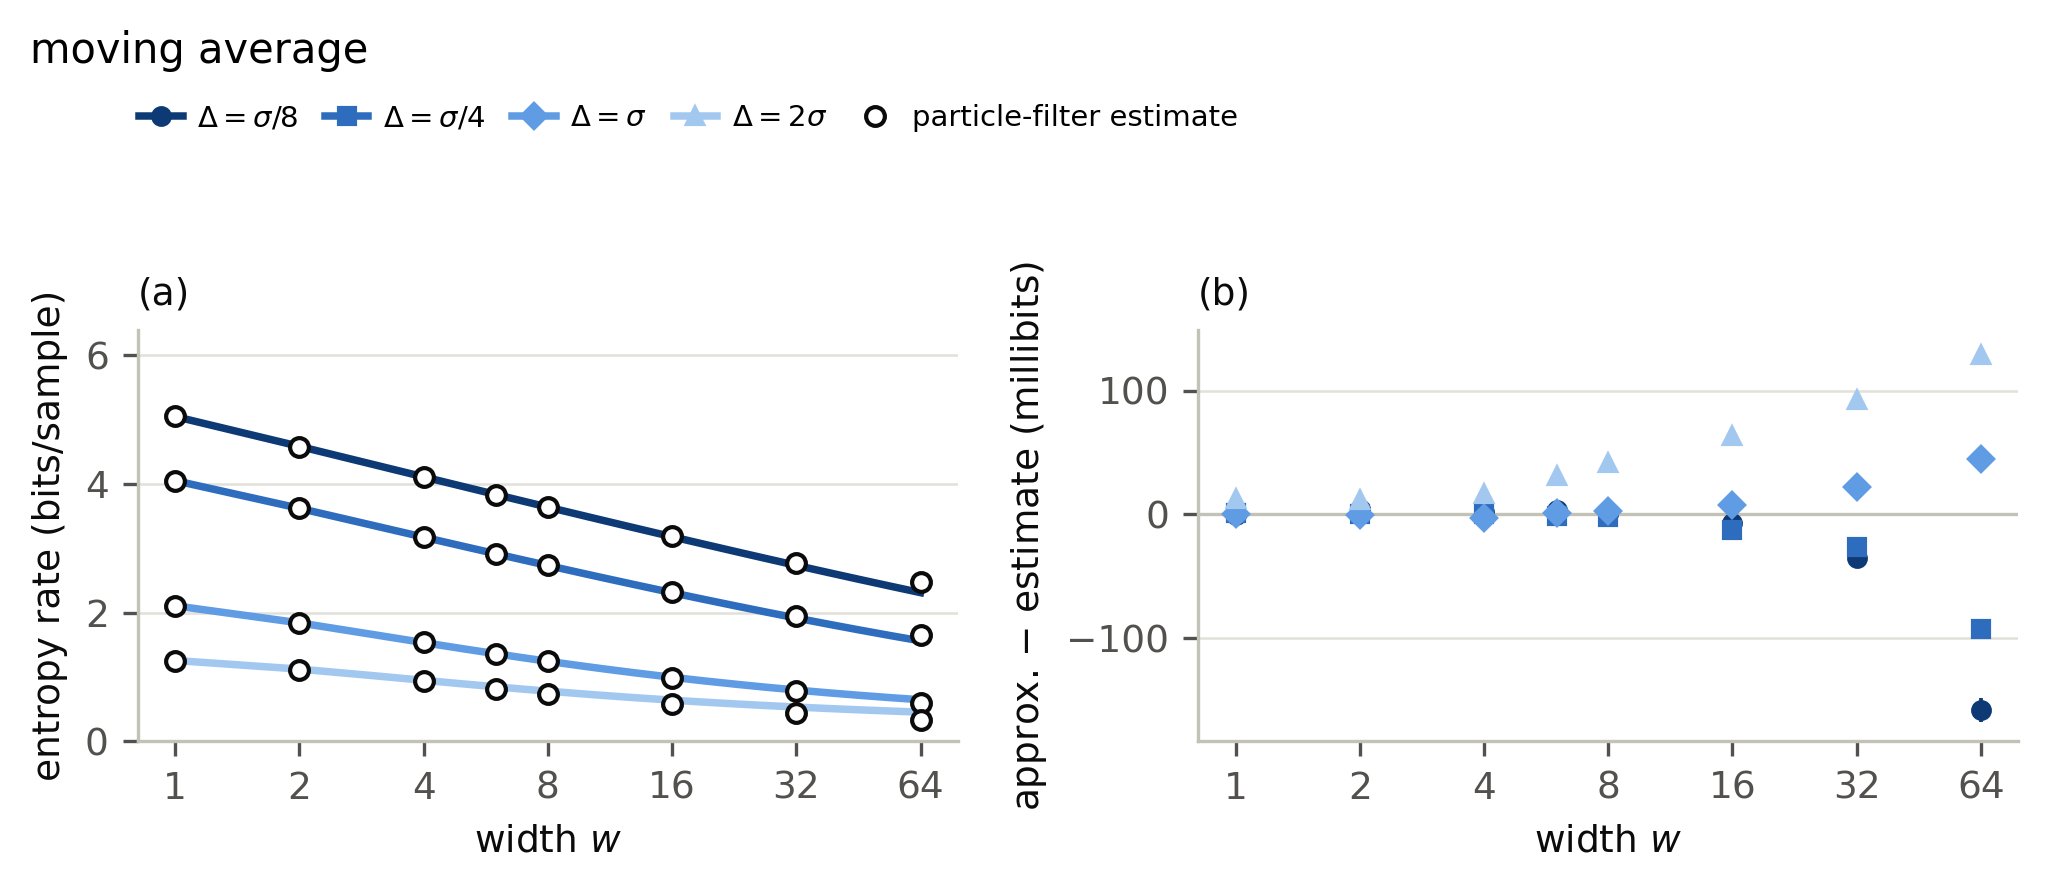
\includegraphics[width=\linewidth]{../experiments/figures/fig_family_ma.png}
\caption{The moving average of width $w$ ($\sigma = 1$). (a) The entropy rate: the analytical approximation on a dense grid of widths (curves) at four quantization steps, with the particle-filter estimates overlaid (open circles; error bars are smaller than the markers). (b) The error of the approximation (approximation minus estimate, in millibits per sample) at the measured points, $\pm$ one standard error. Note that the vertical scale of panel (b) differs from one family to the next.}
\label{fig:4}
\end{figure}

\begin{figure}[t]
\centering
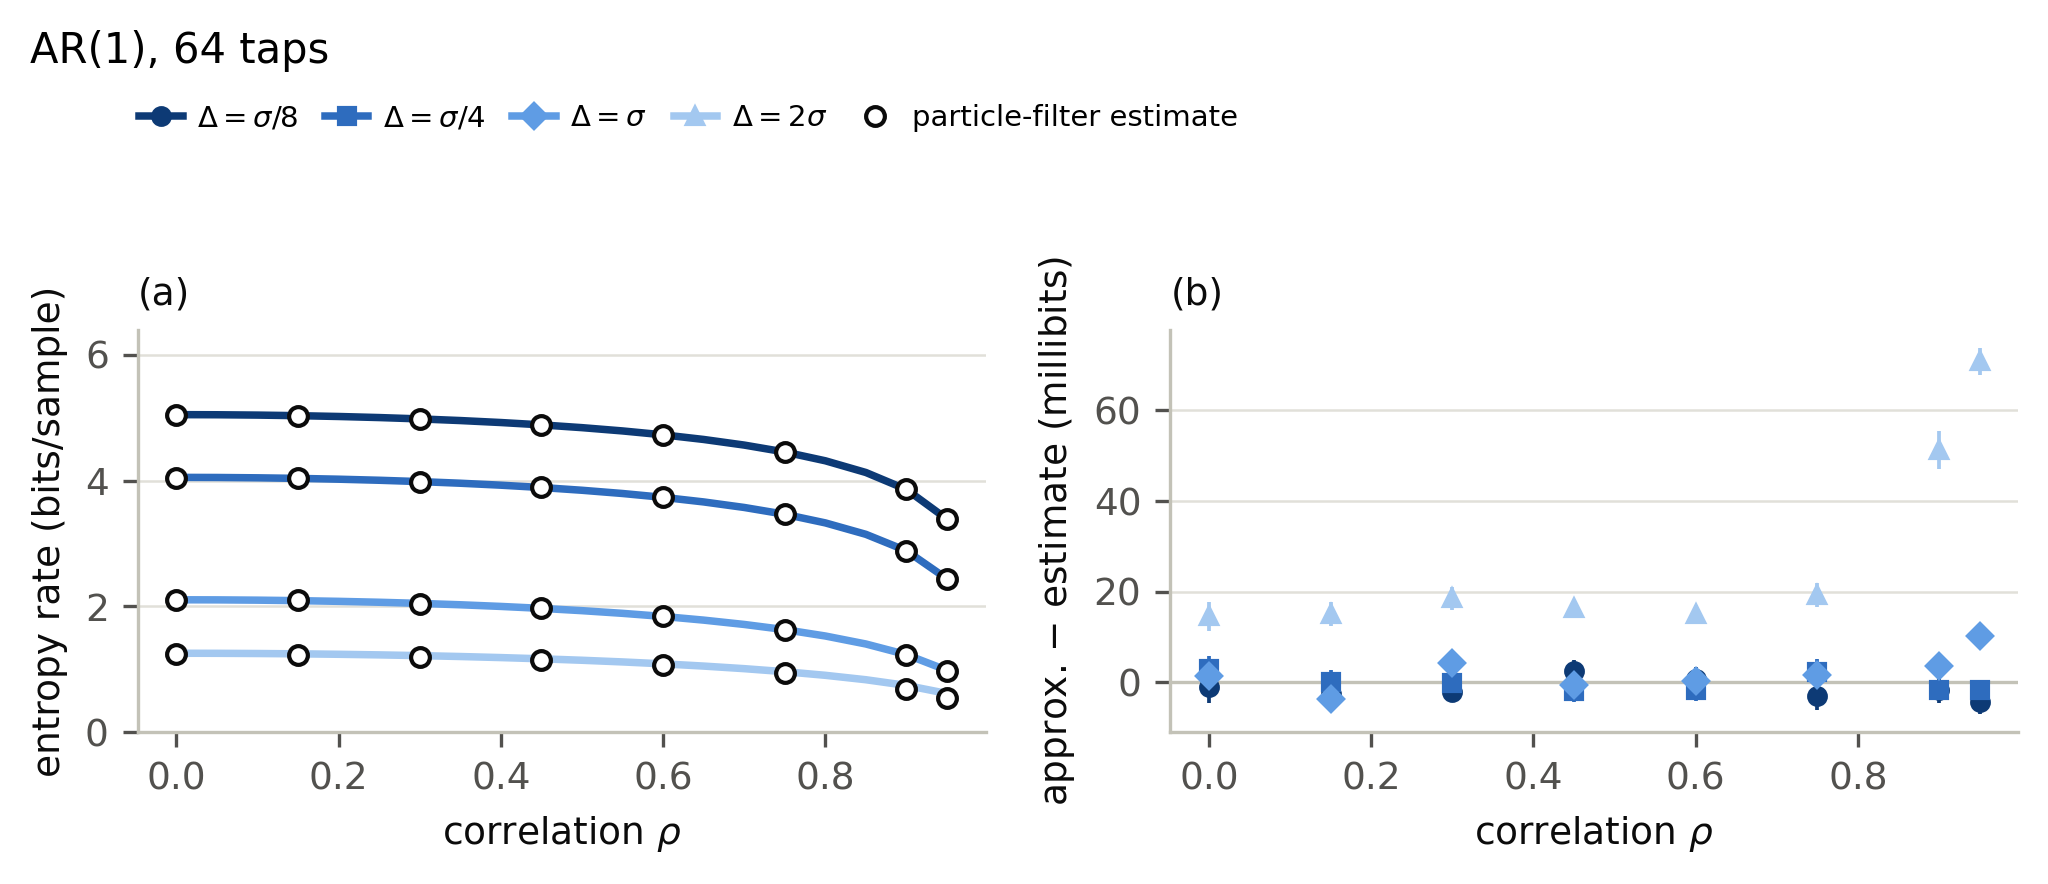
\includegraphics[width=\linewidth]{../experiments/figures/fig_family_ar1.png}
\caption{The AR(1) process with correlation $\rho$, truncated to 64 taps, in the format of Figure 4.}
\label{fig:5}
\end{figure}

\begin{figure}[t]
\centering
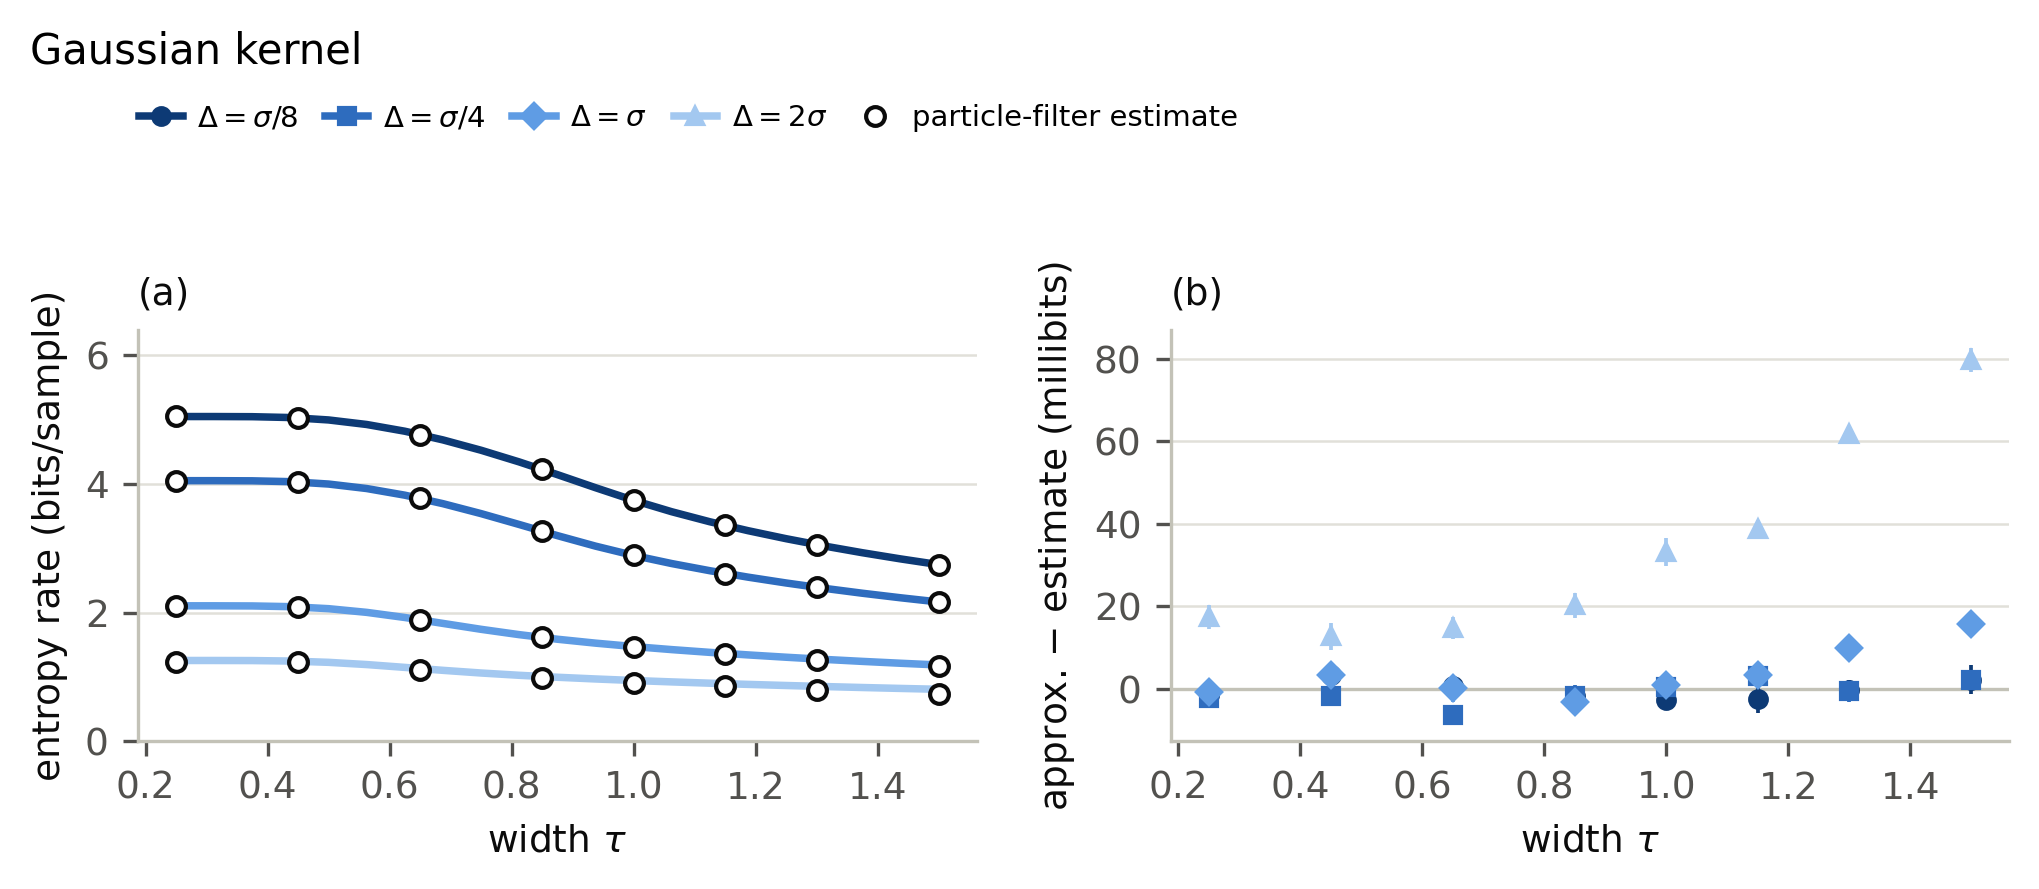
\includegraphics[width=\linewidth]{../experiments/figures/fig_family_gaussian.png}
\caption{The Gaussian kernel of width $\tau$, with $2\lceil 4\tau\rceil + 1$ taps, in the format of Figure 4.}
\label{fig:6}
\end{figure}

\begin{figure}[t]
\centering
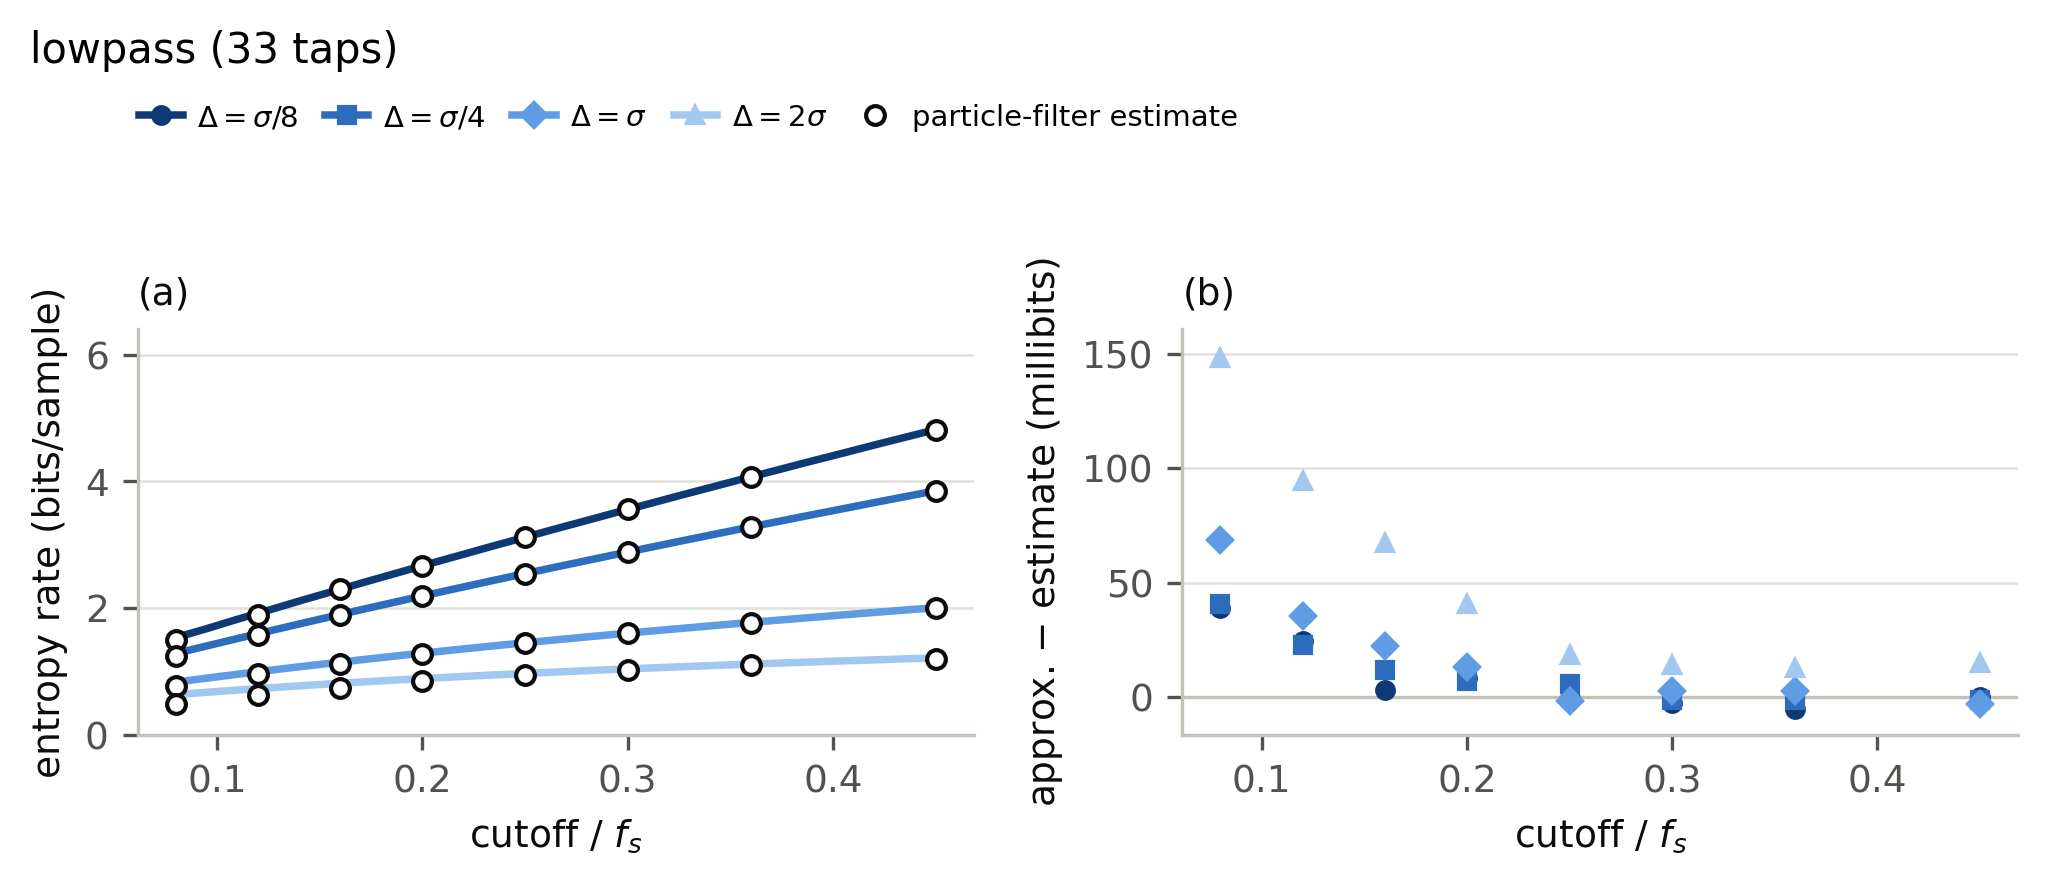
\includegraphics[width=\linewidth]{../experiments/figures/fig_family_lowpass.png}
\caption{The windowed-sinc lowpass filter with 33 taps, as a function of the cutoff frequency, in the format of Figure 4.}
\label{fig:7}
\end{figure}

The filter parameters follow the convergence study of Section 5.1, with the particle count set from the one-step prediction error \(h_0\) of each point, since it is \(h_0\) that governs how hard the filtering problem is: \(N = 8000\) where \(h_0 > 0.3\sigma\), \(N = 30000\) below that, and \(N = 130000\) where \(h_0 < 0.05\sigma\), namely at the lowest four lowpass cutoffs. Sixteen replicates of length \(n = 10000\) are run at every point, reduced to \(n = 5000\) at the hardest ones. Since the particle count needed to keep a replicate locked grows with the sequence length, while the precision of the reported mean depends only on the total sample count (Section 5.1), the shorter replicates buy the same precision at a much lower particle count; we verified directly that the shortening introduces no finite-\(n\) bias. Each point uses independently seeded sequences, so the scatter in the error panels is independent from point to point, and the per-point parameters together with the complete numerical values are recorded in the tables of Appendix C. For white noise the symbol probabilities are available in closed form and the likelihood is computed exactly, so that comparison contains no filter error at all.

For \(\Delta \le \sigma\) the estimates fall on the curves throughout, across families, parameter values, and quantization steps, and the rate panels show no visible discrepancy. The error panels resolve what the rate panels cannot. Over most of each sweep the measured error is within a few millibits of zero, against standard errors of about 3 millibits, so most of this scatter is the noise of the estimator rather than error of the formula. Toward the strongly smoothing end of each sweep a systematic overestimate develops, in the direction predicted by the analysis of Section 3.4. It is clearest for the lowpass family, whose error grows from a few millibits at the wider cutoffs to some tens of millibits at the lowest cutoff, roughly five percent of the rate there; restricted to cutoffs of \(0.2 f_s\) and above, the same family agrees to within \(13\) millibits at every step up to \(\sigma\).

At \(\Delta = 2\sigma\) the overestimate becomes systematic in every family and grows with the strength of the smoothing, from 12 to 15 millibits for white noise, the first difference, and the weakly correlated ends of the sweeps, to about 25 percent of the rate for the lowpass at its lowest cutoff. This is the onset of the coarse-quantization failure anticipated in Section 3.5, and it is why the curves in the rate panels visibly separate from the estimates only at this step.

The moving average is a partial exception, and the one place in these experiments where the comparison is limited by the estimator rather than by the formula. Through width 8 it behaves like the other families, agreeing to within a few millibits for \(\Delta \le \sigma\). At the wider kernels and the finer steps, however, the estimate lies systematically \emph{above} the approximation, by more than a hundred millibits at \(w = 64\) and \(\Delta = \sigma/8\). Since both methods are biased upward, a negative measured error of this size cannot be an error of the approximation, and must instead be residual bias of the filter. A separate sweep of the particle count at that point confirms this reading and shows how slow the convergence is, the estimate still decreasing at \(N = 400000\). This is consistent with the finding of Section 5.1 that the moving average is by far the most biased family for the filter, and it means that these particular points neither confirm nor contradict the approximation. Elsewhere in the sweep, and in every other family, the filter is converged and the comparison is meaningful.

Figure 8 carries the comparison for white noise and the first difference out to \(\Delta = 4\sigma\). The estimates track the curves to within about 5 millibits through \(\Delta = \sigma\) and fall below them by 13 to 14 millibits at \(2\sigma\). At \(4\sigma\) the failure is qualitative, the error being about \(0.34\) bits, larger than the rate itself. Indeed, for white noise the approximation can also be checked against the exact marginal entropy, and its true error is below \(0.01\) millibits for \(\Delta \le \sigma\); the differences measured at the fine steps are therefore attributable to the estimator, not the formula, and they calibrate the residual scatter seen in the other families. As \(\Delta \to \infty\) the error approaches the constant floor \(\tfrac12\log_2(2\pi e/12) \approx 0.255\) bits discussed in Section 3.5, and it does so slowly from above, since the residual spectral term of the formula decays only as \(O(\sigma^2/\Delta^2)\) while the true rate vanishes faster.

\begin{figure}[t]
\centering
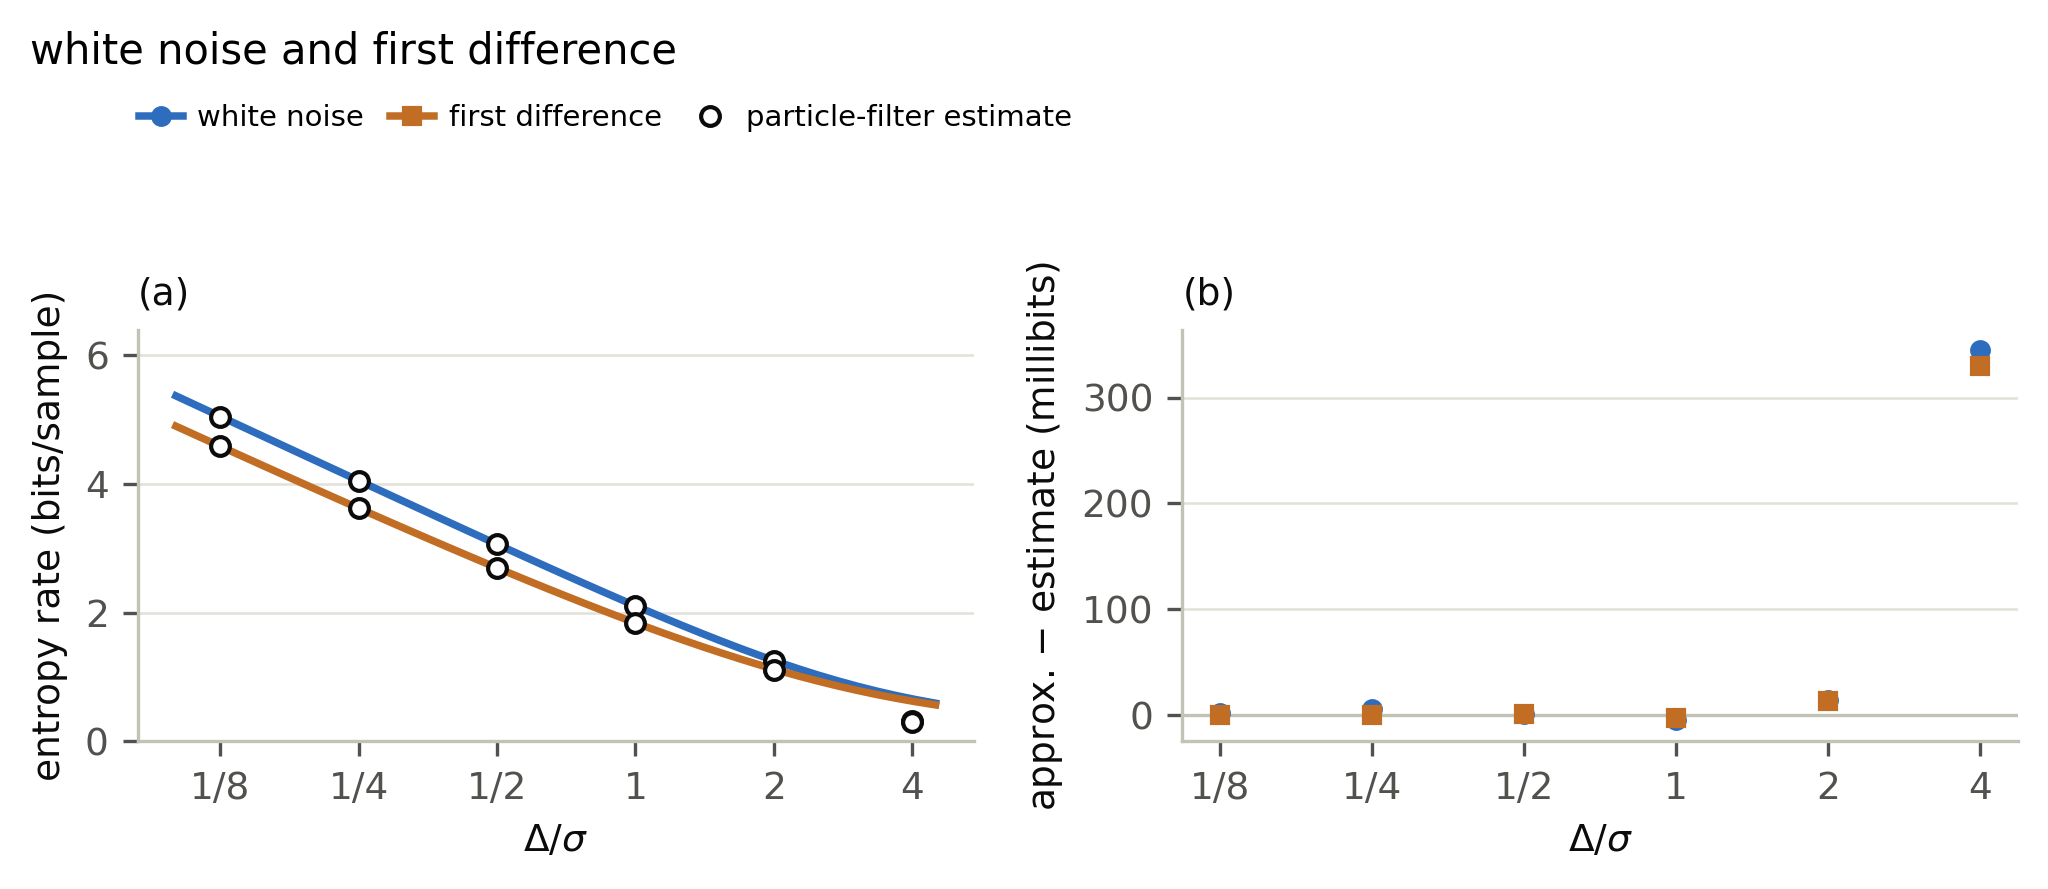
\includegraphics[width=\linewidth]{../experiments/figures/fig_family_whitediff.png}
\caption{White noise and the first difference $[1, -1]$ as functions of the quantization step. (a) The entropy rate: the analytical approximation (curves) with the particle-filter estimates overlaid (open circles); for white noise the likelihood is computed exactly rather than filtered. (b) The error of the approximation at the measured points, $\pm$ one standard error. The rightmost points show the coarse-quantization failure of the approximation.}
\label{fig:8}
\end{figure}

With the accuracy for \(\Delta \le \sigma\) established, the rate panels may also be read as a survey of the dependence of the entropy rate on the process and quantization parameters, mapped densely at negligible cost. In the fine-quantization regime the rate is governed by the one-step prediction error, \(\bar H \approx \tfrac12\log_2(2\pi e\,h_0^2/\Delta^2)\), so the family parameter acts on the rate through \(h_0\). For the moving average \(h_0 = \sigma/\sqrt{w}\), and the top curve of Figure 4(a) falls by very nearly half a bit per doubling of the width; for the lowpass filter the rate is approximately linear in the cutoff, reflecting the bandwidth factor in the Kolmogorov--Szegő integral. The vertical separation between adjacent curves equals \(\log_2\) of the ratio of the steps as long as the quantization is fine relative to the whole spectrum; under strong smoothing part of the spectrum falls below the quantization noise power \(\Delta^2/12\) and the separation compresses, which is visible at the wide end of the moving-average and Gaussian sweeps.

In summary, the approximation agrees with the estimator to within a few millibits per sample for \(\Delta \lesssim \sigma\) over most of every family, including strongly filtered processes on which the classical formula fails outright, and it costs milliseconds rather than the minutes to hours of the estimator. The agreement degrades gradually as the smoothing strengthens, reaching a few percent of the rate at the most strongly filtered points tested, and sharply beyond \(\Delta \approx 2\sigma\), where the additive-noise model of quantization breaks down. In the regime of the target application (\(\sigma/\Delta \approx 4\)) the approximation may be used in place of the estimator for most purposes; beyond \(\Delta \approx 2\sigma\) it should not be used at all, and the estimator remains available there.

\subsection{Comparison with practical compressors}\label{comparison-with-practical-compressors}

Finally, we compare two representative lossless coders against the entropy rate, to indicate how close practical compression comes to the ideal limit; the full codec comparison is deferred to the companion applied paper. The first coder is zlib\footnote{\url{https://zlib.net}} (level 9) applied to the raw symbol stream serialized as little-endian 16-bit integers, representative of the common practice of running a general-purpose byte-oriented compressor over the data as stored. The second is a predictive pipeline: the fixed-point linear predictor of the accompanying package (FLAC style, order 32 for every family, the maximum order of FLAC \cite{RFC9639}) followed by an ANS entropy coder\footnote{The simple-ans package, \url{https://github.com/flatironinstitute/simple_ans}} on the residuals. Each configuration compresses five independent realizations of length \(n = 10^6\), the reference rate being the analytical approximation, which Section 5.2 validated in this range of steps. Figure 9 shows two representative families and Table 2 reports all seven at \(\Delta = \sigma/4\).

\begin{figure}[t]
\centering
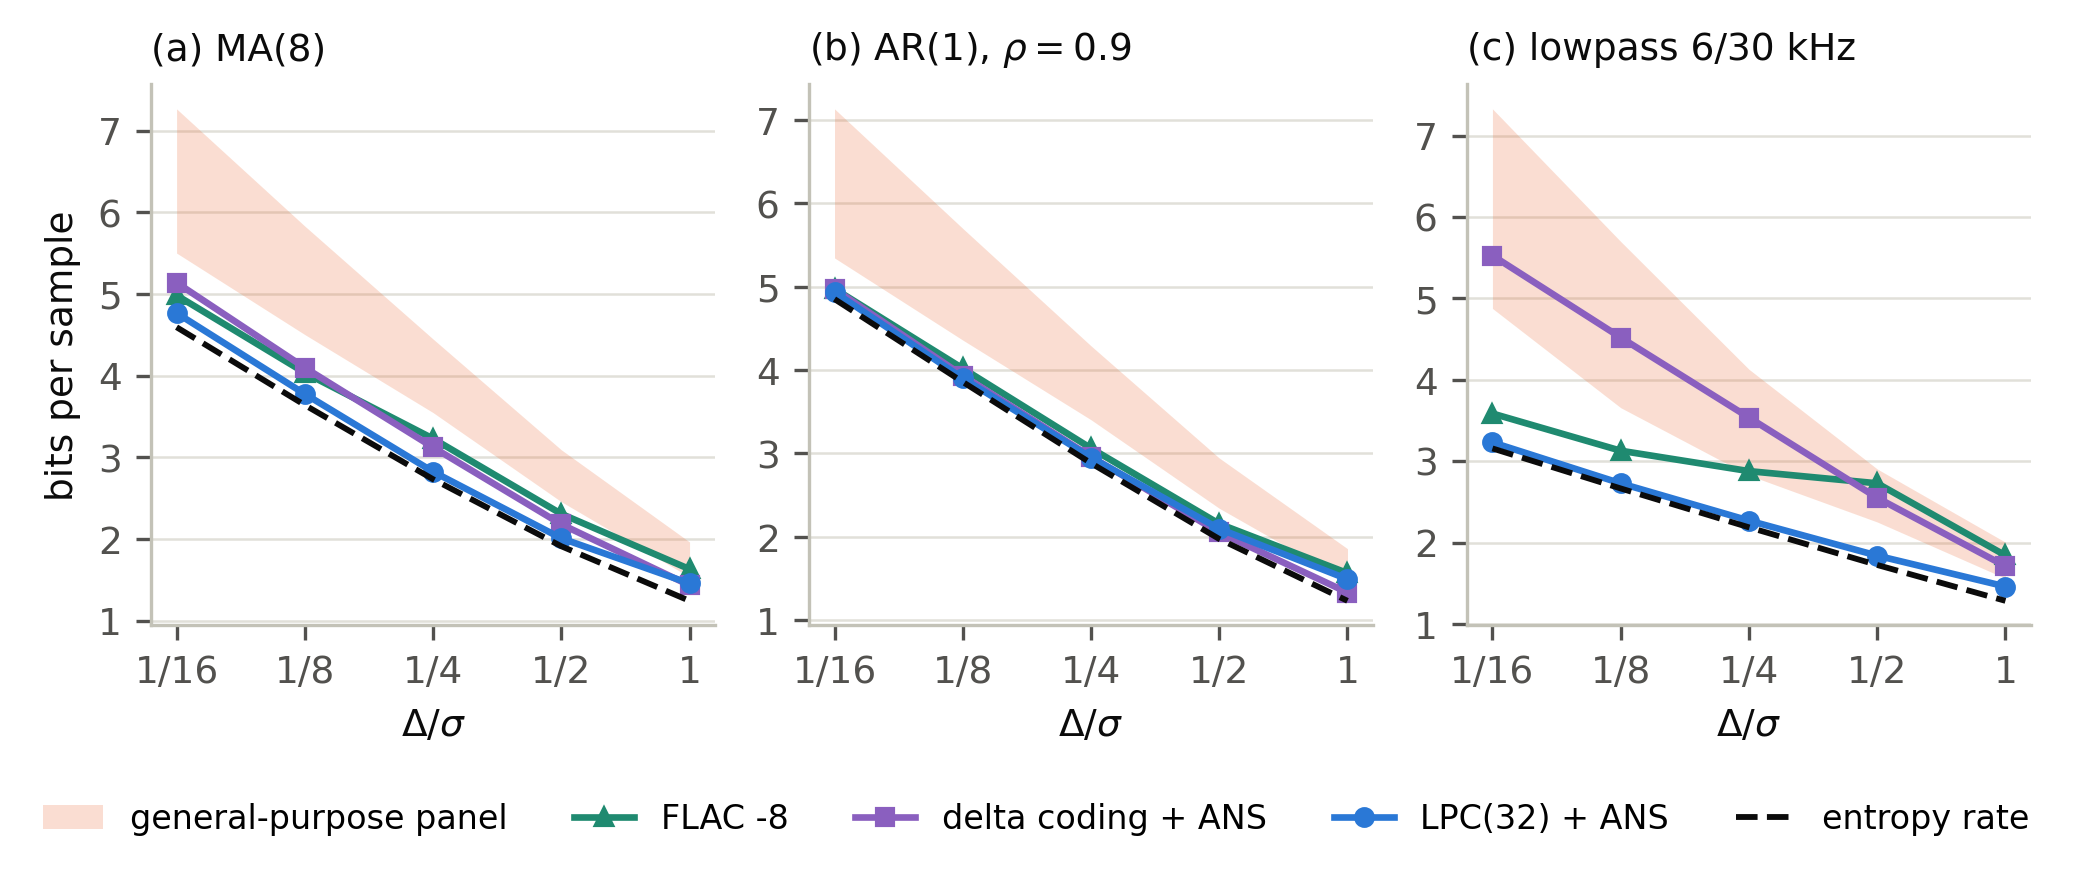
\includegraphics[width=\linewidth]{../experiments/figures/fig_compressors.png}
\caption{Two practical coders against the entropy rate (dashed), for (a) the AR(1) process and (b) the lowpass process, as a function of the quantization step. Each point is the mean over five realizations of length $n = 10^6$; the spread across realizations is smaller than the markers.}
\label{fig:9}
\end{figure}

\textbf{Table 2.} Bits per sample achieved by the two coders at \(\Delta = \sigma/4\), against the entropy rate and the order-0 (memoryless) symbol entropy, with the overhead relative to the entropy rate in parentheses. Note that the order-0 entropy is the same for every family, since the marginal distribution does not depend on the correlation structure.

\begin{longtable}[]{@{}lrrrr@{}}
\toprule\noalign{}
process & entropy rate & order-0 & LPC(32) + ANS & zlib on raw \\
\midrule\noalign{}
\endhead
\bottomrule\noalign{}
\endlastfoot
white & 4.051 & 4.049 & 4.114 (+1.6\%) & 5.484 (+35\%) \\
first difference & 3.621 & 4.049 & 3.687 (+1.8\%) & 5.229 (+44\%) \\
MA(8) & 2.731 & 4.048 & 2.824 (+3.4\%) & 4.449 (+63\%) \\
AR(1), \(\rho=0.9\) & 2.884 & 4.047 & 2.952 (+2.4\%) & 4.291 (+49\%) \\
Gaussian, \(\tau=1\) & 2.888 & 4.049 & 2.957 (+2.4\%) & 4.564 (+58\%) \\
Gaussian, \(\tau=1.5\) & 2.165 & 4.049 & 2.242 (+3.6\%) & 3.745 (+73\%) \\
lowpass 6/30 kHz & 2.188 & 4.049 & 2.271 (+3.8\%) & 4.130 (+89\%) \\
\end{longtable}

The predictive pipeline comes within 2 to 4 percent of the entropy rate at \(\Delta = \sigma/4\) for every family, and its performance is similar at the finer steps. The gap widens as the quantization coarsens, reaching roughly 6 to 21 percent at \(\Delta = \sigma\), presumably because prediction from rounded values becomes less effective and the residual retains structure that the memoryless entropy coder cannot exploit. For white noise, where there is nothing to predict, ANS alone on the raw stream is within about one percent of the rate at every step.

The predictor order matters more than might be expected. With the seemingly natural choice of order \(L - 1\), matched to the length of the generating kernel, the MA(8) overhead at \(\Delta = \sigma/4\) is 0.32 bits per sample rather than 0.09, and the first difference behaves similarly. These are the families whose spectra have exact zeros, so their AR representations decay slowly and useful prediction requires an order well beyond the kernel length; at order 32 the excess is largely gone. The smooth families are insensitive to this choice.

The byte-oriented coder is far from the limit throughout, 35 to 89 percent above the rate at \(\Delta = \sigma/4\), and worst for the strongly smoothed families, which are precisely the ones with the most structure to exploit. Indeed, at this step zlib compresses the lowpass process to more bits than its memoryless entropy, so it fails to realize even the gains available to a symbol-by-symbol code. In other words, the compressibility of these signals resides almost entirely in the correlation structure, and a coder must model that structure explicitly to approach the limit.

\section{Implementation}\label{implementation}

Three implementations accompany the paper; the repository is cited as an artifact. \emph{{[}Repository reference and final package name to be added.{]}}

The first is a standalone Python package implementing the full pipeline: process specification by preset, convolution kernel, or autocovariance; the cepstral minimum-phase factorization with its diagnostics; the fully adapted filter with the collapse diagnostic; the analytical approximation; and the compression benchmark. A command-line interface produces the estimates (streaming replicates with a running mean and standard error, with the approximation reported alongside) and the plots.

The second is a WebGPU compute shader. The filter is implemented as a single WGSL kernel, with one workgroup per replicate and particles vectorized within it. The same shader source is executed both from Python (via WebGPU bindings) and natively in the browser. Because WebGPU lacks double precision, the log-space normal CDF and its inverse were rebuilt in single precision; the per-step increments are accumulated in double precision on the host, where the collapse diagnostic is applied unchanged.

The third is an interactive web application that exposes the method interactively: the user adjusts the process (filter) and the quantizer and observes the estimated rate, the analytical approximation, and real codec performance in response.

\section{Discussion}\label{discussion}

We have presented an analytical approximation to the entropy rate of a uniformly quantized stationary Gaussian process, together with a particle-filter method for estimating the exact rate. The approximation replaces the spectrum \(S\) in the classical high-resolution formula with \(S + \Delta^2/12\), the exact spectral density of the dithered process, and thereby remains finite and accurate for the bandlimited and strongly filtered processes on which the classical formula fails. The estimator follows the route established for the information rates of channels with memory \cite{ArnoldEtAl2006,DauwelsLoeliger2008}, reducing the rate to the log-likelihood of a filter evaluated on a single long typical sequence; its components (minimum-phase spectral factorization, the hidden Markov structure it induces, and the fully adapted particle filter that the model admits in closed form) are standard, and the contribution is the manner in which they are combined into a practical method that works at all quantization scales.

The method has several limitations, each of which is a candidate for future work. The lattice error in the Riemann-sum step is expressed exactly as a Poisson sum but is not quantified; bounding it would turn the approximation into a controlled estimate in the fine-to-moderate regime. The slack in the Gaussian entropy upper bound for the dithered process, namely the per-sample non-Gaussianity of \(X + U\), is likewise not quantified. Note that both errors push the formula upward. In the extreme coarse regime the constant floor of the formula is an artifact of the additive-noise model, and the formula should not be used there. The estimator, for its part, requires the process to be purely nondeterministic (Section 4.2), so the strictly bandlimited case, in which \(S\) vanishes on a set of positive measure, is served only by the approximation; its leading behavior there is correct, matching the information dimension rate of Geiger and Koch \cite{GeigerKoch2019}, but its accuracy at finite \(\Delta\) has not been tested here, since the spectra of Section 5 are positive almost everywhere. Finally, the development is restricted to Gaussian processes; extensions to non-Gaussian sources would broaden the applicability.

A companion applied paper will use these tools to evaluate compression algorithms on real noisy scientific data against the ideal limit computed here.

\appendix

\section{Numerically stable filter arithmetic}\label{numerically-stable-filter-arithmetic}

When an observation falls in a far tail relative to a particle's prediction, \(\Phi(r) - \Phi(l)\) underflows in double precision, so the filter works in log space throughout using \(\mathrm{log\_ndtr} = \ln\Phi\):

\[\ln\alpha = \mathrm{log\_ndtr}(b) + \ln\!\big(1 - e^{\,\mathrm{log\_ndtr}(a) - \mathrm{log\_ndtr}(b)}\big),\]

evaluating \(\ln(1-e^x)\) as \(\ln(-\mathrm{expm1}(x))\) for \(x > -\ln 2\) and as \(\mathrm{log1p}(-e^x)\) otherwise. Here \((a,b) = (-r,-l)\) when \(l + r > 0\) and \((l,r)\) otherwise, using the reflection \(\Phi(r) - \Phi(l) = \Phi(-l) - \Phi(-r)\). Reflecting on the sign of the midpoint guarantees \(a + b \le 0\), which keeps \(\mathrm{log\_ndtr}\) out of the saturated region where two nearly equal values near \(0\) cancel. The likelihood increment (step 2 of the algorithm) is accumulated with a log-sum-exp.

The truncated-normal draw (step 4) uses the same reflection and the inverse of \(\mathrm{log\_ndtr}\) rather than a generic truncated-normal routine:

\[w = \mathrm{ndtri\_exp}\big(\mathrm{logaddexp}(\ln\Phi(a),\; \ln U + \ln\alpha)\big), \qquad U \sim \mathrm{Unif}(0,1),\]

then undoes the reflection and clips to \([l,r)\) as a guard. Since \(\ln\Phi(a)\) and \(\ln\alpha\) are already available from the weight computation, the entire step costs one \(\mathrm{log\_ndtr}\) pair and one \(\mathrm{ndtri\_exp}\) per particle; these transcendental evaluations dominate the runtime.

\section{Filter collapse and its diagnostic}\label{filter-collapse-and-its-diagnostic}

Under fine quantization (\(h_0 \ll \sigma\), \(\Delta \lesssim h_0\)) the state is nearly determined by the observations. If the particle cloud drifts off by more than a cell, each particle is forced to draw an extreme innovation, which the near-unit-circle inverse filter amplifies into a worse error at the next step. Past some point every particle is wrong simultaneously, and the resulting estimate is invalid rather than merely noisy.

The effective sample size does not detect this failure, since the surviving particles agree with one another whether or not they agree with the data; the ESS therefore remains healthy through a collapse. A diagnostic that does work is based on the per-step likelihood increment itself. A particle whose prediction is \(d\) standard deviations from the observed cell contributes about \(\log(\Delta/h_0) - d^2/2\) nats, so a filter that is tracking the state cannot fall far below \(\log\min(1, \Delta/h_0)\) per step, and a step falling tens of nats below that level indicates a loss of lock rather than an unlucky symbol. Note that the scale term matters: under fine quantization every step is legitimately worth about \(\log(\Delta/h_0)\) nats, so a fixed threshold would produce false alarms. Replicates that lose lock are discarded rather than averaged, and a run with no surviving replicates reports a collapse instead of an estimate. Since the spectral approximation of Section 3 shares no machinery with the filter, it also serves as an independent check on every reported result.

\section{Detailed comparison tables}\label{detailed-comparison-tables}

The tables below record every Monte Carlo point of the comparison of Section 5.2: the particle-filter estimate (mean $\pm$ standard error over the replicates), the analytical approximation, and their difference in millibits per sample, together with the particle count $N$, sequence length $n$, and replicate count $r$ used at each point. An entry marked \emph{discarded} lost lock in the indicated number of replicates and is provisional in the sense of Section 5.1; an entry marked \emph{collapsed} had no surviving replicate. The tables are generated directly from the results files in the accompanying repository.

{\small
\begin{longtable}[]{@{}rrrrrrrr@{}}
\toprule\noalign{}
width $w$ & $\Delta/\sigma$ & $N$ & $n$ & $r$ & estimate (bits/sample) & approximation & error (millibits) \\
\midrule\noalign{}
\endhead
\bottomrule\noalign{}
\caption{\textbf{moving average}. The particle-filter estimate against the analytical approximation (error is approximation minus estimate), with the particle count $N$, sequence length $n$, and replicate count $r$ used at each point.}\label{tab:family1}\\
\endlastfoot
1 & 0.125 & 8000 & 10000 & 16 & 5.0490 $\pm$ 0.0020 & 5.0480 & -1.0 \\
1 & 0.25 & 8000 & 10000 & 16 & 4.0501 $\pm$ 0.0025 & 4.0508 & +0.7 \\
1 & 1 & 8000 & 10000 & 16 & 2.1045 $\pm$ 0.0027 & 2.1048 & +0.3 \\
1 & 2 & 8000 & 10000 & 16 & 1.2422 $\pm$ 0.0022 & 1.2546 & +12.4 \\
2 & 0.125 & 8000 & 10000 & 16 & 4.5795 $\pm$ 0.0025 & 4.5839 & +4.4 \\
2 & 0.25 & 8000 & 10000 & 16 & 3.6202 $\pm$ 0.0027 & 3.6207 & +0.4 \\
2 & 1 & 8000 & 10000 & 16 & 1.8400 $\pm$ 0.0025 & 1.8396 & -0.4 \\
2 & 2 & 8000 & 10000 & 16 & 1.1091 $\pm$ 0.0026 & 1.1208 & +11.7 \\
4 & 0.125 & 8000 & 10000 & 16 & 4.1082 $\pm$ 0.0021 & 4.1099 & +1.7 \\
4 & 0.25 & 8000 & 10000 & 16 & 3.1720 $\pm$ 0.0031 & 3.1725 & +0.4 \\
4 & 1 & 8000 & 10000 & 16 & 1.5355 $\pm$ 0.0032 & 1.5327 & -2.7 \\
4 & 2 & 8000 & 10000 & 16 & 0.9299 $\pm$ 0.0028 & 0.9462 & +16.4 \\
6 & 0.125 & 8000 & 10000 & 16 & 3.8304 $\pm$ 0.0021 & 3.8339 & +3.4 \\
6 & 0.25 & 8000 & 10000 & 16 & 2.9139 $\pm$ 0.0026 & 2.9127 & -1.2 \\
6 & 1 & 8000 & 10000 & 16 & 1.3575 $\pm$ 0.0029 & 1.3585 & +0.9 \\
6 & 2 & 8000 & 10000 & 16 & 0.8138 $\pm$ 0.0035 & 0.8449 & +31.1 \\
8 & 0.125 & 8000 & 10000 & 16 & 3.6390 $\pm$ 0.0024 & 3.6395 & +0.5 \\
8 & 0.25 & 8000 & 10000 & 16 & 2.7333 $\pm$ 0.0025 & 2.7313 & -2.0 \\
8 & 1 & 8000 & 10000 & 16 & 1.2390 $\pm$ 0.0021 & 1.2420 & +3.0 \\
8 & 2 & 8000 & 10000 & 16 & 0.7366 $\pm$ 0.0035 & 0.7777 & +41.1 \\
16 & 0.125 & 30000 & 10000 & 16 & 3.1860 $\pm$ 0.0023 & 3.1789 & -7.1 \\
16 & 0.25 & 30000 & 10000 & 16 & 2.3217 $\pm$ 0.0030 & 2.3090 & -12.7 \\
16 & 1 & 30000 & 10000 & 16 & 0.9858 $\pm$ 0.0021 & 0.9935 & +7.6 \\
16 & 2 & 30000 & 10000 & 16 & 0.5743 $\pm$ 0.0021 & 0.6378 & +63.5 \\
32 & 0.125 & 30000 & 10000 & 16 & 2.7692 $\pm$ 0.0035 & 2.7336 & -35.6 \\
32 & 0.25 & 30000 & 10000 & 16 & 1.9420 $\pm$ 0.0014 & 1.9152 & -26.8 \\
32 & 1 & 30000 & 10000 & 16 & 0.7729 $\pm$ 0.0028 & 0.7951 & +22.2 \\
32 & 2 & 30000 & 10000 & 16 & 0.4380 $\pm$ 0.0036 & 0.5306 & +92.6 \\
64 & 0.125 & 30000 & 10000 & 16 & 2.4681 $\pm$ 0.0100 & 2.3098 & -158.3 \\
64 & 0.25 & 30000 & 10000 & 16 & 1.6527 $\pm$ 0.0052 & 1.5596 & -93.1 \\
64 & 1 & 30000 & 10000 & 16 & 0.5993 $\pm$ 0.0028 & 0.6441 & +44.8 \\
64 & 2 & 30000 & 10000 & 16 & 0.3226 $\pm$ 0.0052 & 0.4516 & +129.0 \\
\end{longtable}
}

{\small
\begin{longtable}[]{@{}rrrrrrrr@{}}
\toprule\noalign{}
correlation $\rho$ & $\Delta/\sigma$ & $N$ & $n$ & $r$ & estimate (bits/sample) & approximation & error (millibits) \\
\midrule\noalign{}
\endhead
\bottomrule\noalign{}
\caption{\textbf{AR(1), 64 taps}. The particle-filter estimate against the analytical approximation (error is approximation minus estimate), with the particle count $N$, sequence length $n$, and replicate count $r$ used at each point.}\label{tab:family2}\\
\endlastfoot
0 & 0.125 & 8000 & 10000 & 16 & 5.0490 $\pm$ 0.0035 & 5.0480 & -1.0 \\
0 & 0.25 & 8000 & 10000 & 16 & 4.0480 $\pm$ 0.0029 & 4.0508 & +2.9 \\
0 & 1 & 8000 & 10000 & 16 & 2.1034 $\pm$ 0.0026 & 2.1048 & +1.4 \\
0 & 2 & 8000 & 10000 & 16 & 1.2401 $\pm$ 0.0032 & 1.2546 & +14.5 \\
0.15 & 0.125 & 8000 & 10000 & 16 & 5.0343 $\pm$ 0.0025 & 5.0317 & -2.6 \\
0.15 & 0.25 & 8000 & 10000 & 16 & 4.0346 $\pm$ 0.0028 & 4.0346 & +0.0 \\
0.15 & 1 & 8000 & 10000 & 16 & 2.0946 $\pm$ 0.0024 & 2.0909 & -3.7 \\
0.15 & 2 & 8000 & 10000 & 16 & 1.2304 $\pm$ 0.0026 & 1.2454 & +15.0 \\
0.3 & 0.125 & 8000 & 10000 & 16 & 4.9824 $\pm$ 0.0017 & 4.9802 & -2.2 \\
0.3 & 0.25 & 8000 & 10000 & 16 & 3.9836 $\pm$ 0.0024 & 3.9835 & -0.0 \\
0.3 & 1 & 8000 & 10000 & 16 & 2.0429 $\pm$ 0.0028 & 2.0472 & +4.4 \\
0.3 & 2 & 8000 & 10000 & 16 & 1.1984 $\pm$ 0.0025 & 1.2169 & +18.5 \\
0.45 & 0.125 & 8000 & 10000 & 16 & 4.8828 $\pm$ 0.0025 & 4.8853 & +2.5 \\
0.45 & 0.25 & 8000 & 10000 & 16 & 3.8915 $\pm$ 0.0023 & 3.8895 & -2.0 \\
0.45 & 1 & 8000 & 10000 & 16 & 1.9687 $\pm$ 0.0017 & 1.9680 & -0.7 \\
0.45 & 2 & 8000 & 10000 & 16 & 1.1496 $\pm$ 0.0016 & 1.1660 & +16.4 \\
0.6 & 0.125 & 8000 & 10000 & 16 & 4.7264 $\pm$ 0.0026 & 4.7272 & +0.8 \\
0.6 & 0.25 & 8000 & 10000 & 16 & 3.7348 $\pm$ 0.0024 & 3.7331 & -1.7 \\
0.6 & 1 & 8000 & 10000 & 16 & 1.8393 $\pm$ 0.0024 & 1.8396 & +0.3 \\
0.6 & 2 & 8000 & 10000 & 16 & 1.0710 $\pm$ 0.0020 & 1.0860 & +15.0 \\
0.75 & 0.125 & 8000 & 10000 & 16 & 4.4572 $\pm$ 0.0031 & 4.4541 & -3.0 \\
0.75 & 0.25 & 8000 & 10000 & 16 & 3.4618 $\pm$ 0.0029 & 3.4640 & +2.2 \\
0.75 & 1 & 8000 & 10000 & 16 & 1.6282 $\pm$ 0.0023 & 1.6298 & +1.6 \\
0.75 & 2 & 8000 & 10000 & 16 & 0.9421 $\pm$ 0.0027 & 0.9614 & +19.3 \\
0.9 & 0.125 & 8000 & 10000 & 16 & 3.8597 $\pm$ 0.0028 & 3.8580 & -1.7 \\
0.9 & 0.25 & 8000 & 10000 & 16 & 2.8854 $\pm$ 0.0018 & 2.8837 & -1.7 \\
0.9 & 1 & 8000 & 10000 & 16 & 1.2294 $\pm$ 0.0016 & 1.2329 & +3.5 \\
0.9 & 2 & 8000 & 10000 & 16 & 0.6920 $\pm$ 0.0042 & 0.7432 & +51.2 \\
0.95 & 0.125 & 8000 & 10000 & 16 & 3.3913 $\pm$ 0.0025 & 3.3869 & -4.4 \\
0.95 & 0.25 & 8000 & 10000 & 16 & 2.4389 $\pm$ 0.0023 & 2.4372 & -1.7 \\
0.95 & 1 & 8000 & 10000 & 16 & 0.9731 $\pm$ 0.0023 & 0.9833 & +10.2 \\
0.95 & 2 & 8000 & 10000 & 16 & 0.5442 $\pm$ 0.0030 & 0.6150 & +70.7 \\
\end{longtable}
}

{\small
\begin{longtable}[]{@{}rrrrrrrr@{}}
\toprule\noalign{}
width $\tau$ & $\Delta/\sigma$ & $N$ & $n$ & $r$ & estimate (bits/sample) & approximation & error (millibits) \\
\midrule\noalign{}
\endhead
\bottomrule\noalign{}
\caption{\textbf{Gaussian kernel}. The particle-filter estimate against the analytical approximation (error is approximation minus estimate), with the particle count $N$, sequence length $n$, and replicate count $r$ used at each point.}\label{tab:family3}\\
\endlastfoot
0.25 & 0.125 & 8000 & 10000 & 16 & 5.0495 $\pm$ 0.0023 & 5.0480 & -1.4 \\
0.25 & 0.25 & 8000 & 10000 & 16 & 4.0530 $\pm$ 0.0021 & 4.0508 & -2.2 \\
0.25 & 1 & 8000 & 10000 & 16 & 2.1055 $\pm$ 0.0029 & 2.1048 & -0.7 \\
0.25 & 2 & 8000 & 10000 & 16 & 1.2372 $\pm$ 0.0029 & 1.2546 & +17.5 \\
0.45 & 0.125 & 8000 & 10000 & 16 & 5.0239 $\pm$ 0.0027 & 5.0274 & +3.5 \\
0.45 & 0.25 & 8000 & 10000 & 16 & 4.0320 $\pm$ 0.0026 & 4.0303 & -1.7 \\
0.45 & 1 & 8000 & 10000 & 16 & 2.0840 $\pm$ 0.0030 & 2.0873 & +3.2 \\
0.45 & 2 & 8000 & 10000 & 16 & 1.2304 $\pm$ 0.0034 & 1.2431 & +12.7 \\
0.65 & 0.125 & 8000 & 10000 & 16 & 4.7684 $\pm$ 0.0023 & 4.7691 & +0.6 \\
0.65 & 0.25 & 8000 & 10000 & 16 & 3.7818 $\pm$ 0.0019 & 3.7756 & -6.3 \\
0.65 & 1 & 8000 & 10000 & 16 & 1.8871 $\pm$ 0.0033 & 1.8872 & +0.1 \\
0.65 & 2 & 8000 & 10000 & 16 & 1.1139 $\pm$ 0.0027 & 1.1286 & +14.7 \\
0.85 & 0.125 & 8000 & 10000 & 16 & 4.2271 $\pm$ 0.0023 & 4.2255 & -1.6 \\
0.85 & 0.25 & 8000 & 10000 & 16 & 3.2672 $\pm$ 0.0029 & 3.2653 & -1.8 \\
0.85 & 1 & 8000 & 10000 & 16 & 1.6155 $\pm$ 0.0015 & 1.6124 & -3.1 \\
0.85 & 2 & 8000 & 10000 & 16 & 0.9853 $\pm$ 0.0030 & 1.0056 & +20.2 \\
1 & 0.125 & 8000 & 10000 & 16 & 3.7481 $\pm$ 0.0016 & 3.7453 & -2.8 \\
1 & 0.25 & 8000 & 10000 & 16 & 2.8880 $\pm$ 0.0026 & 2.8884 & +0.3 \\
1 & 1 & 8000 & 10000 & 16 & 1.4704 $\pm$ 0.0026 & 1.4713 & +1.0 \\
1 & 2 & 8000 & 10000 & 16 & 0.9103 $\pm$ 0.0035 & 0.9434 & +33.2 \\
1.15 & 0.125 & 30000 & 10000 & 16 & 3.3572 $\pm$ 0.0034 & 3.3547 & -2.5 \\
1.15 & 0.25 & 30000 & 10000 & 16 & 2.6065 $\pm$ 0.0029 & 2.6095 & +3.1 \\
1.15 & 1 & 30000 & 10000 & 16 & 1.3613 $\pm$ 0.0018 & 1.3647 & +3.4 \\
1.15 & 2 & 30000 & 10000 & 16 & 0.8552 $\pm$ 0.0021 & 0.8940 & +38.8 \\
1.3 & 0.125 & 30000 & 10000 & 16 & 3.0572 $\pm$ 0.0021 & 3.0569 & -0.3 \\
1.3 & 0.25 & 30000 & 10000 & 16 & 2.3934 $\pm$ 0.0027 & 2.3930 & -0.4 \\
1.3 & 1 & 30000 & 10000 & 16 & 1.2684 $\pm$ 0.0026 & 1.2782 & +9.9 \\
1.3 & 2 & 30000 & 10000 & 16 & 0.7908 $\pm$ 0.0018 & 0.8527 & +61.9 \\
1.5 & 0.125 & 30000 & 10000 & 16 & 2.7434 $\pm$ 0.0035 & 2.7457 & +2.3 \\
1.5 & 0.25 & 30000 & 10000 & 16 & 2.1625 $\pm$ 0.0024 & 2.1646 & +2.1 \\
1.5 & 1 & 30000 & 10000 & 16 & 1.1689 $\pm$ 0.0020 & 1.1847 & +15.8 \\
1.5 & 2 & 30000 & 10000 & 16 & 0.7271 $\pm$ 0.0029 & 0.8068 & +79.7 \\
\end{longtable}
}

{\small
\begin{longtable}[]{@{}rrrrrrrr@{}}
\toprule\noalign{}
cutoff / $f_s$ & $\Delta/\sigma$ & $N$ & $n$ & $r$ & estimate (bits/sample) & approximation & error (millibits) \\
\midrule\noalign{}
\endhead
\bottomrule\noalign{}
\caption{\textbf{lowpass, 33 taps}. The particle-filter estimate against the analytical approximation (error is approximation minus estimate), with the particle count $N$, sequence length $n$, and replicate count $r$ used at each point.}\label{tab:family4}\\
\endlastfoot
0.08 & 0.125 & 130000 & 5000 & 16 & 1.4923 $\pm$ 0.0017 & 1.5311 & +38.8 \\
0.08 & 0.25 & 130000 & 5000 & 16 & 1.2417 $\pm$ 0.0023 & 1.2821 & +40.4 \\
0.08 & 1 & 130000 & 5000 & 16 & 0.7601 $\pm$ 0.0027 & 0.8285 & +68.4 \\
0.08 & 2 & 130000 & 5000 & 16 & 0.4820 $\pm$ 0.0044 & 0.6302 & +148.2 \\
0.12 & 0.125 & 130000 & 5000 & 16 & 1.8912 $\pm$ 0.0026 & 1.9158 & +24.6 \\
0.12 & 0.25 & 130000 & 5000 & 16 & 1.5713 $\pm$ 0.0027 & 1.5940 & +22.7 \\
0.12 & 1 & 130000 & 5000 & 16 & 0.9570 $\pm$ 0.0033 & 0.9926 & +35.5 \\
0.12 & 2 & 130000 & 5000 & 16 & 0.6315 $\pm$ 0.0029 & 0.7261 & +94.6 \\
0.16 & 0.125 & 260000 & 5000 & 16 & 2.2916 $\pm$ 0.0032 & 2.2945 & +2.9 \\
0.16 & 0.25 & 130000 & 5000 & 16 & 1.8840 $\pm$ 0.0023 & 1.8957 & +11.7 \\
0.16 & 1 & 130000 & 5000 & 16 & 1.1221 $\pm$ 0.0024 & 1.1443 & +22.3 \\
0.16 & 2 & 130000 & 5000 & 16 & 0.7425 $\pm$ 0.0033 & 0.8098 & +67.4 \\
0.2 & 0.125 & 130000 & 5000 & 16 & 2.6573 $\pm$ 0.0035 & 2.6658 & +8.5 \\
0.2 & 0.25 & 130000 & 5000 & 16 & 2.1811 $\pm$ 0.0038 & 2.1882 & +7.1 \\
0.2 & 1 & 130000 & 5000 & 16 & 1.2721 $\pm$ 0.0029 & 1.2853 & +13.2 \\
0.2 & 2 & 130000 & 5000 & 16 & 0.8430 $\pm$ 0.0033 & 0.8837 & +40.7 \\
0.25 & 0.125 & 130000 & 5000 & 16 & 3.1159 $\pm$ 0.0027 & 3.1154 & -0.5 \\
0.25 & 0.25 & 130000 & 5000 & 16 & 2.5357 $\pm$ 0.0041 & 2.5413 & +5.6 \\
0.25 & 1 & 130000 & 5000 & 16 & 1.4510 $\pm$ 0.0030 & 1.4492 & -1.8 \\
0.25 & 2 & 130000 & 5000 & 16 & 0.9470 $\pm$ 0.0035 & 0.9651 & +18.1 \\
0.3 & 0.125 & 130000 & 5000 & 16 & 3.5584 $\pm$ 0.0042 & 3.5557 & -2.8 \\
0.3 & 0.25 & 130000 & 5000 & 16 & 2.8842 $\pm$ 0.0034 & 2.8830 & -1.2 \\
0.3 & 1 & 130000 & 5000 & 16 & 1.5987 $\pm$ 0.0029 & 1.6012 & +2.5 \\
0.3 & 2 & 130000 & 5000 & 16 & 1.0227 $\pm$ 0.0030 & 1.0368 & +14.1 \\
0.36 & 0.125 & 30000 & 10000 & 16 & 4.0751 $\pm$ 0.0030 & 4.0697 & -5.4 \\
0.36 & 0.25 & 30000 & 10000 & 16 & 3.2804 $\pm$ 0.0026 & 3.2791 & -1.3 \\
0.36 & 1 & 30000 & 10000 & 16 & 1.7682 $\pm$ 0.0020 & 1.7707 & +2.5 \\
0.36 & 2 & 30000 & 10000 & 16 & 1.1001 $\pm$ 0.0015 & 1.1126 & +12.5 \\
0.45 & 0.125 & 8000 & 10000 & 16 & 4.8154 $\pm$ 0.0029 & 4.8155 & +0.0 \\
0.45 & 0.25 & 8000 & 10000 & 16 & 3.8500 $\pm$ 0.0024 & 3.8489 & -1.1 \\
0.45 & 1 & 8000 & 10000 & 16 & 2.0062 $\pm$ 0.0022 & 2.0030 & -3.2 \\
0.45 & 2 & 8000 & 10000 & 16 & 1.1950 $\pm$ 0.0019 & 1.2100 & +15.0 \\
\end{longtable}
}

{\small
\begin{longtable}[]{@{}lrrrrrrr@{}}
\toprule\noalign{}
process & $\Delta/\sigma$ & $N$ & $n$ & $r$ & estimate (bits/sample) & approximation & error (millibits) \\
\midrule\noalign{}
\endhead
\bottomrule\noalign{}
\caption{\textbf{White noise and first difference}. The particle-filter estimate against the analytical approximation over the quantization step (error is approximation minus estimate).}\label{tab:family5}\\
\endlastfoot
white noise & 0.125 & 8000 & 10000 & 16 & 5.0466 $\pm$ 0.0021 & 5.0480 & +1.4 \\
white noise & 0.25 & 8000 & 10000 & 16 & 4.0456 $\pm$ 0.0030 & 4.0508 & +5.2 \\
white noise & 0.5 & 8000 & 10000 & 16 & 3.0610 $\pm$ 0.0028 & 3.0620 & +1.0 \\
white noise & 1 & 8000 & 10000 & 16 & 2.1094 $\pm$ 0.0025 & 2.1048 & -4.6 \\
white noise & 2 & 8000 & 10000 & 16 & 1.2407 $\pm$ 0.0029 & 1.2546 & +13.9 \\
white noise & 4 & 8000 & 10000 & 16 & 0.3136 $\pm$ 0.0019 & 0.6583 & +344.7 \\
first difference & 0.125 & 8000 & 10000 & 16 & 4.5843 $\pm$ 0.0020 & 4.5839 & -0.4 \\
first difference & 0.25 & 8000 & 10000 & 16 & 3.6205 $\pm$ 0.0027 & 3.6207 & +0.2 \\
first difference & 0.5 & 8000 & 10000 & 16 & 2.6929 $\pm$ 0.0028 & 2.6941 & +1.2 \\
first difference & 1 & 8000 & 10000 & 16 & 1.8423 $\pm$ 0.0030 & 1.8396 & -2.8 \\
first difference & 2 & 8000 & 10000 & 16 & 1.1077 $\pm$ 0.0026 & 1.1208 & +13.1 \\
first difference & 4 & 8000 & 10000 & 16 & 0.2923 $\pm$ 0.0031 & 0.6226 & +330.3 \\
\end{longtable}
}


\begin{thebibliography}{99}

\bibitem{GrayNeuhoff1998}
R.~M. Gray and D.~L. Neuhoff, ``Quantization,'' \emph{IEEE Transactions on
Information Theory}, vol.~44, no.~6, pp.~2325--2383, 1998.

\bibitem{GrayStockham1993}
R.~M. Gray and T.~G. Stockham, Jr., ``Dithered quantizers,'' \emph{IEEE
Transactions on Information Theory}, vol.~39, no.~3, pp.~805--812, 1993.

\bibitem{ZamirFeder1996}
R.~Zamir and M.~Feder, ``Information rates of pre/post-filtered dithered
quantizers,'' \emph{IEEE Transactions on Information Theory}, vol.~42, no.~5,
pp.~1340--1353, 1996.

\bibitem{GrenanderSzego1958}
U.~Grenander and G.~Szeg\H{o}, \emph{Toeplitz Forms and Their Applications}.
Berkeley: University of California Press, 1958.

\bibitem{PittShephard1999}
M.~K. Pitt and N.~Shephard, ``Filtering via simulation: auxiliary particle
filters,'' \emph{Journal of the American Statistical Association}, vol.~94,
no.~446, pp.~590--599, 1999.

\bibitem{GeigerKoch2019}
B.~C. Geiger and T.~Koch, ``On the information dimension of stochastic
processes,'' \emph{IEEE Transactions on Information Theory}, vol.~65,
no.~10, pp.~6496--6518, 2019.

\bibitem{ArnoldEtAl2006}
D.~M. Arnold, H.-A. Loeliger, P.~O. Vontobel, A.~Kav\v{c}i\'c, and W.~Zeng,
``Simulation-based computation of information rates for channels with
memory,'' \emph{IEEE Transactions on Information Theory}, vol.~52, no.~8,
pp.~3498--3508, 2006.

\bibitem{DauwelsLoeliger2008}
J.~Dauwels and H.-A. Loeliger, ``Computation of information rates by particle
methods,'' \emph{IEEE Transactions on Information Theory}, vol.~54, no.~1,
pp.~406--409, 2008.

\bibitem{CoverThomas2006}
T.~M. Cover and J.~A. Thomas, \emph{Elements of Information Theory}, 2nd~ed.
Hoboken, NJ: Wiley, 2006.

\bibitem{GishPierce1968}
H.~Gish and J.~Pierce, ``Asymptotically efficient quantizing,''
\emph{IEEE Transactions on Information Theory}, vol.~14, no.~5,
pp.~676--683, 1968.

\bibitem{Chung1961}
K.~L. Chung, ``A note on the ergodic theorem of information theory,''
\emph{Annals of Mathematical Statistics}, vol.~32, no.~2, pp.~612--614, 1961.

\bibitem{OppenheimSchafer2010}
A.~V. Oppenheim and R.~W. Schafer, \emph{Discrete-Time Signal Processing},
3rd~ed. Upper Saddle River, NJ: Prentice-Hall, 2010.

\bibitem{DelMoral2004}
P.~Del Moral, \emph{Feynman--Kac Formulae: Genealogical and Interacting
Particle Systems with Applications}. New York: Springer, 2004.

\bibitem{RFC9639}
M.~Q.~C. van Beurden and A.~Weaver, ``Free Lossless Audio Codec (FLAC),''
RFC~9639, RFC Editor, Dec. 2024.

\end{thebibliography}

\end{document}
